\chapter{Experiments}
\label{ch-experiments}

This chapter examines the estimation accuracy, runtime performance and scalability of the general \algolpmf\ method and its extensions introduced in \refchapter{\ref{ch-laplace-approximation}} and \refchapter{\ref{ch-rodes}} by comparing with the other state-of-art inference techniques empirically.
In \refsection{\ref{sec-implementation}}, the implementation of the algorithms is discussed.
Then four dynamical systems with different dimensionality and complexity are used for the experiments.
\refsection{\ref{sec-lotka-volterra}} and \refsection{\ref{sec-protein-signalling-transduction-pathway}} consider the state and parameter estimation for deterministic dynamical systems, while \refsection{\ref{sec-lorenz-96}} and \refsection{\ref{sec-lorenz-63}} consider two random dynamical systems.

\section{Implementation}
\label{sec-implementation}

The source code of this work is implemented from the ground up using the general purpose programming language Python 3\footnote{\url{https://www.python.org/}}.
The MATLAB\footnote{\url{https://www.mathworks.com/products/matlab.html}} code for the \algovgmgp\ algorithm from \cite{gorbach2017scalable} is used as the blueprint during implementation.
The advantages the Python implementation includes
\begin{itemize}
    \item The native support of object-oriented programming makes the application interface clean and extensible. Specifically, the \texttt{Dynamical} and \texttt{Kernel} classes are implemented as abstract classes so that new dynamical systems and new kernels can be prototyped quickly.
    \item The language is none proprietary and many Python machine learning libraries are well supported in the open-source community and are widely used in enterprise level applications.
\end{itemize}

Several important open-source packages have made this Python solution possible:
\begin{itemize}
    \item The SciPy\footnote{\url{https://www.scipy.org/}} package provides a powerful optimization module and other I/O utilities to read and write files in MATLAB format.
    \item The NumPy\footnote{\url{http://www.numpy.org/}} package is the backbone for linear algebra operations and random variable generation.
    \item The SymPy\footnote{\url{http://www.sympy.org/en/index.html}} package is used for symbolic mathematics when implementing the general interface for dynamical systems and kernel functions. It is also used to calculate the gradients and Hessians of the cost functions for part of the solution.
    \item The matplotlib\footnote{\url{http://matplotlib.org/}} package helps to produce publication quality plotting.
    \item The Jupyter Notebook\footnote{\url{http://jupyter.org/}} is used as the GUI interface to combine code, visualizations and documentation in a sharable format.
    \item The sdeint\footnote{\url{https://github.com/mattja/sdeint}} package provides the numerical methods to solve SDEs. 
    \item The TensorFlow\footnote{\url{https://www.tensorflow.org/}} package is a machine learning library popular among the deep learning community, which provides auto-differentiation support for part of the solution.
\end{itemize}


\section{Lotka-Volterra model}
\label{sec-lotka-volterra}

The first deterministic dynamical system examined in this chapter is the \emph{Lotka-Volterra} model \citep{lotka1932growth}, which is frequently used in ecology to describe the interaction between the prey species and the predator species over time.
The model consists of two first-order, nonlinear differential equations where the states $x(t), y(t)\in \R_{\geqslant 0}$ are the populations of the prey and the predator respectively at time point $t$.
The ODEs of the model are given by
\begin{align}
    \dot{x}(t) & = \alpha x(t) - \beta x(t)y(t)
    \nonumber
    \\
    \dot{y}(t) & = \delta x(t)y(t) - \gamma y(t)
    \label{eq-lotka-odes}
\end{align}
where $\alpha, \beta, \delta, \gamma \in \R^+$ are the parameters controlling the dynamics.
 

\subsubsection*{Experimental setup}

\begin{table}
\centering
\caption{Experimental setup for the Lotka-Volterra model. The system dimension is denoted by $K$ and the number of observable dimensions is $K_{obs}$. Based on the parameter values $\alpha$, $\beta$, $\delta$, and $\gamma$, the ODEs are integrated from time $t_0$ to $t_T$ with a step size of $\delta t$. The observation noise variance $\dymsigmak{k}^2$ is assumed to be the identical for each state. For each time unit, $freq_{obs}$ denotes the number of observations to be collected, which are equally distributed over the time line.}
\label{table-lotka-setup}
\begin{tabular}{|c|c|c|c|c|c|c|c|c|}
\hline
$K$ & $K_{obs}$ & $t_0$ & $t_T$ & $\delta t$ & $\alpha, \beta, \delta, \gamma$ & $\dymsigmak{k}^2$  & $freq_{obs}$ \\ \hline
2 & 2 & 0 & 2 & 0.01 & 2, 1, 1, 4 & 0.1 & 10 \\ \hline
\end{tabular}
\end{table}

\reftable{\ref{table-lotka-setup}} shows the setup for the experiment.
The experiment is repeated 10 times with each time an independently collected observation set.
Since the \algolpmf\ method is derived from the \algovgmgp\ method, in the following, we compare the results using both methods.
The \algolpmf\ method is run first without any positivity constraint and then it is run again with positivity constraint on the parameters, which are referred to as \algolpmf\ and \algolpmfpos\ respectively.
It would be interesting to constrain both the states and the parameters to be positive, but the inference fails as shown in \reffigure{\ref{fig-lotka-fail}}. 
The reason for that in unclear yet due to time constraints and requires further investigation.
In order to provide a fair comparison in terms of runtime, both methods are deployed on a desktop with an Intel i5 quad-core CPU and 16 GB of memory.

\begin{figure}
    \centering
    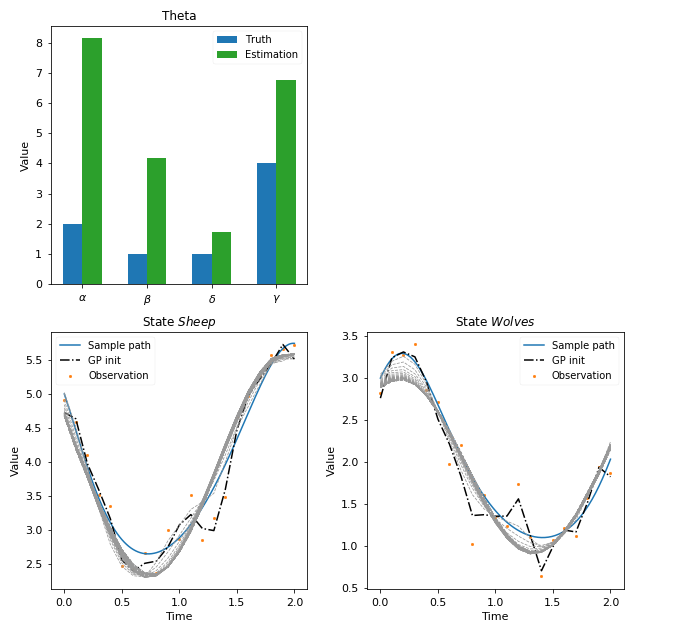
\includegraphics[width=0.8\textwidth]{graphics/lotka-fail}
    \caption{Inference for the Lotka-Volterra model fails when both the states and parameters are constrained to be positive.}
    \label{fig-lotka-fail}
\end{figure}

\subsubsection*{State estimation}

\begin{figure}
    \centering
    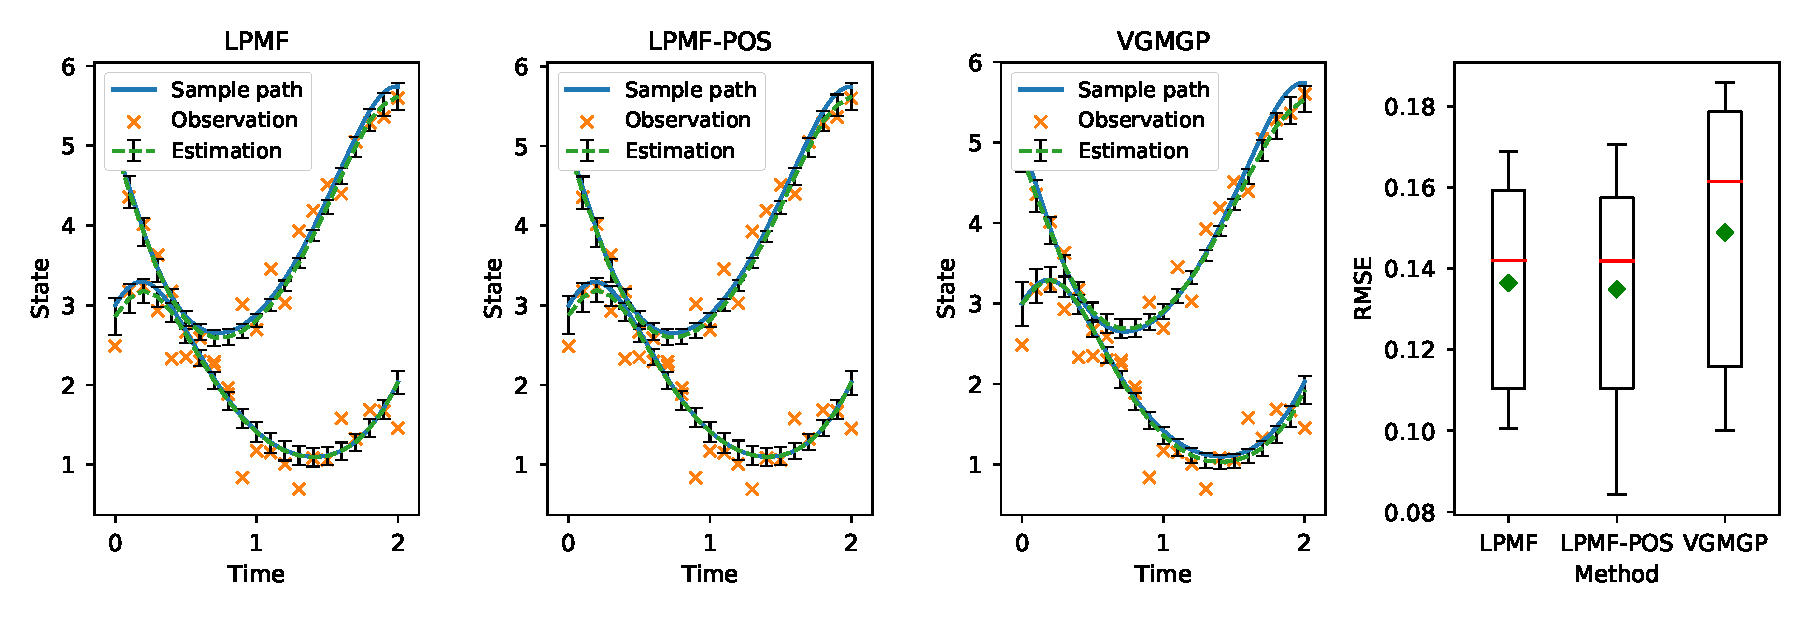
\includegraphics[width=\textwidth]{graphics/lotka-states}
    \caption{State estimation results for the Lotka-Volterra model. The left plot shows the result using \algolpmf; the left middle plot shows the result using \algolpmfpos; the right middle plot shows the result using \algovgmgp; the right plot summarizes the RMSE after 10 independent runs. The error bars in the first three plots indicate one standard deviation.}
    \label{fig-lotka-state}
\end{figure}

\reffigure{\ref{fig-lotka-state}} shows the results after the 10 independent runs.
For illustration purposes, the observations from one run is also plotted to indicate the noise level.
The dotted green lines are obtained by averaging the means of the state estimation for the 10 runs, while the error bars indicate one standard deviation of the means.
The figure shows that the state estimation results are very close to each other and is almost identical to the ground truth.

To quantify the accuracy, the root mean square error (RMSE) is used and is defined as follows:
\begin{align}
    RMSE
    & = \frac{1}{K}\sum_{k}{\sqrt{
        \frac{1}{N}\sum_{n=1}^N{
            (\dymxhatktn{k}{n} - \dymxktn{k}{n})^2
        }
    }}    
\end{align}
where $K$ indicates the number of states, $N$ is the total number of observations for each dimension, and $\dymxhatktn{k}{n}$ and $\dymxktn{k}{n}$ are the predicted and true values for the $k$-th state at time point $t$ respectively.
The RMSEs are very close to each other with the \algolpmf\ method having slightly lower error.

\subsubsection*{Parameter estimation}

\begin{figure}
    \centering
    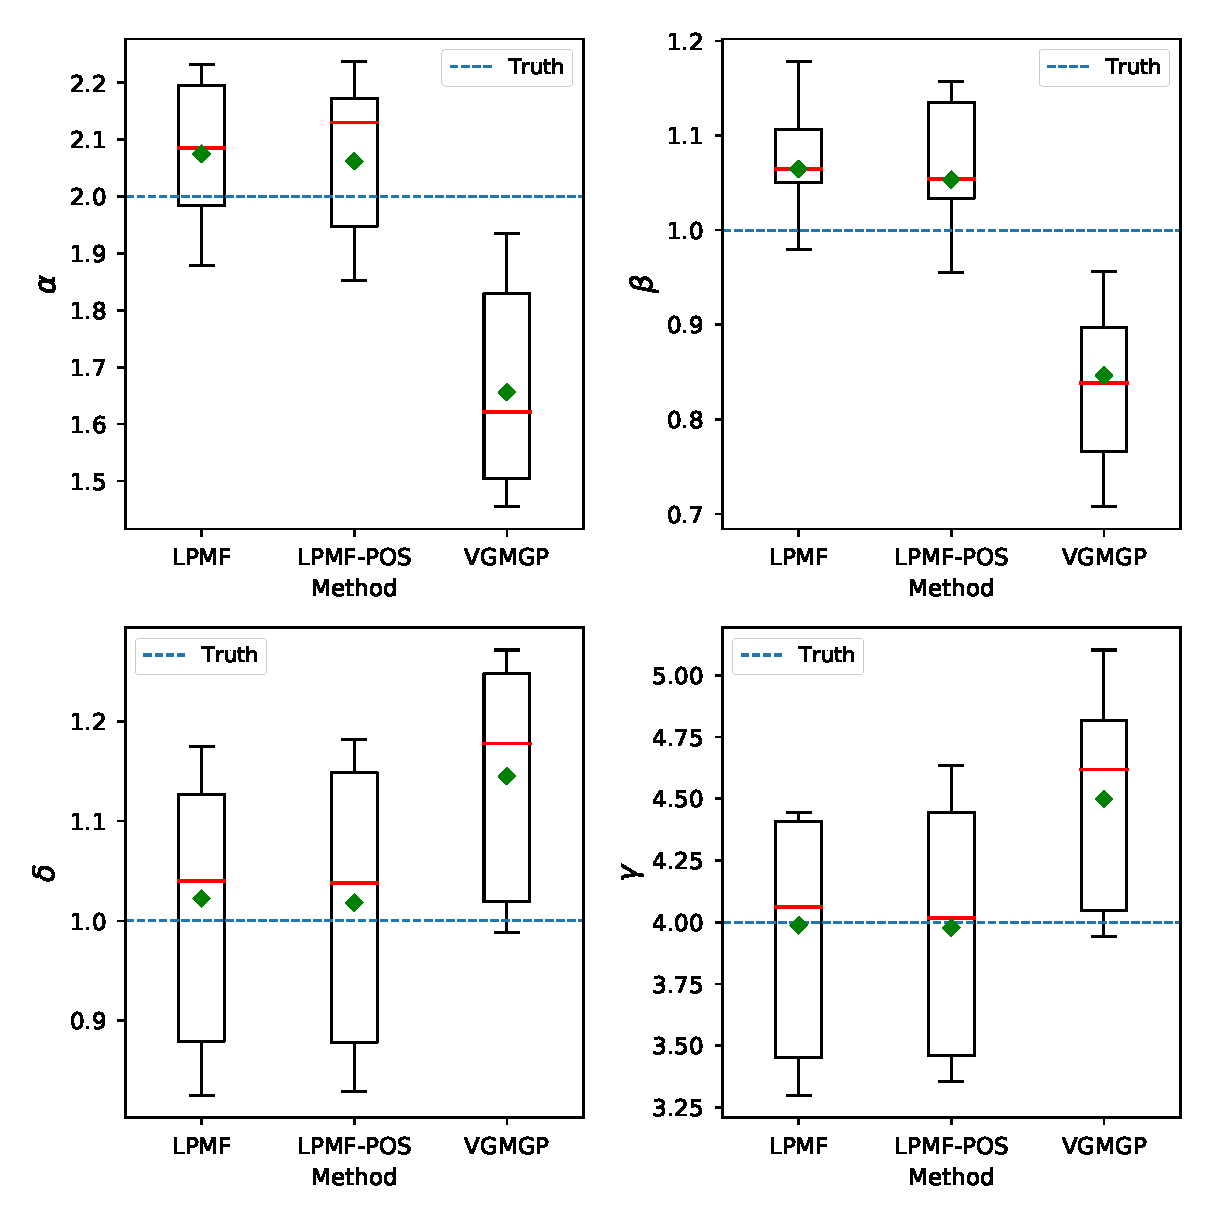
\includegraphics[width=1\textwidth]{graphics/lotka-parameters-boxplot}
    \caption{Parameter estimation results for the Lotka-Volterra model. In the box plot, the median is indicated by the red line, while the mean is shown as the green diamond. The box shows the lower and upper quartiles, while the whiskers are the 5th and 95th percentiles. The true parameter value is shown as the dotted blue line.}
    \label{fig-lotka-parameters-boxplot}
\end{figure}

The estimation results for the parameters of the Lotka-Volterra model are shown in \reffigure{\ref{fig-lotka-parameters-boxplot}}.
The \algolpmf\ method again achieves better results than the \algovgmgp\ algorithm, even with the positivity constraint on the parameters.
The mean values for the prediction from \algolpmf\ are also very close to the true parameter values.

To explain this, first note that both methods assume the decoupling of states from the other states and the decoupling of the states and the parameters when constructing the proxy distribution $Q$.
However, the \algovgmgp\ method further assumes the decoupling of the same states across time points, which is not the case for \algolpmf.
Since the ODEs of the Lotka-Volterra model satisfies the structural assumption, if the conditional distributions in \refequationp{\ref{eq-vgmgp-theta-conditional}} and \refequationp{\ref{eq-vgmgp-xu-conditional}} are indeed Gaussian, then Laplace approximation is expected to correctly find the mode the distribution.

\subsubsection*{Runtime performance}

\begin{figure}
    \centering
    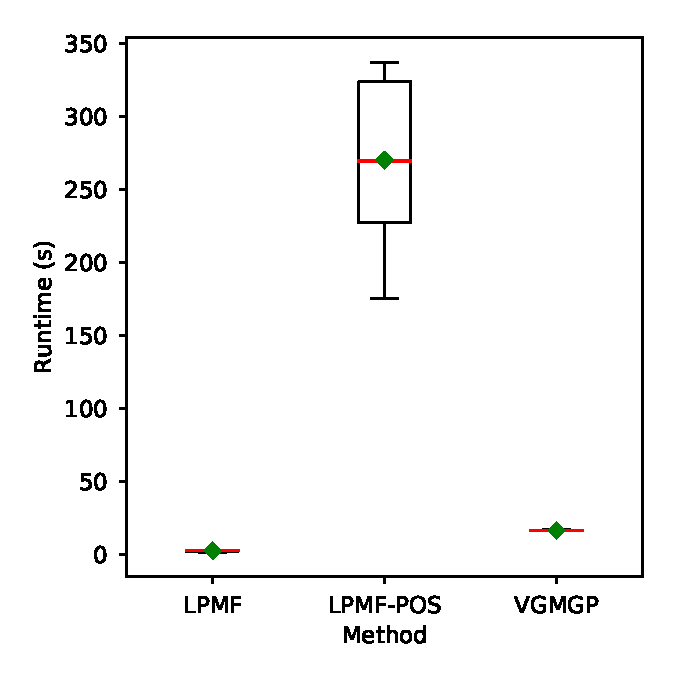
\includegraphics[width=0.48\textwidth]{graphics/lotka-runtime-boxplot}
    \caption{Runtime performance for the Lotka-Volterra model. In the box plot, the median is indicated by the red line, while the mean is shown as the green diamond. The box shows the lower and upper quartiles, while the whiskers are the 5th and 95th percentiles.}
    \label{fig-lotka-runtime-boxplot}
\end{figure}

In terms of runtime, both the \algolpmf\ method when no positivity constraint is imposed and the \algovgmgp\ method are extremely fast.
On average, the \algolpmf\ method finishes in 2.4 seconds and the \algovgmgp\ method completes in 16.3 seconds.
Since \algolpmf\ is implemented in Python while \algovgmgp\ is implemented MATLAB, exact comparison is infeasible.
In general, the \algolpmf\ is likely to be more efficient since the evaluation of the expectations \refequationp{\ref{eq-vgmgp-lambda-vi-optimal}} and \refequationp{\ref{eq-vgmgp-psiu-vi-optimal}} is not required.
Moreover, the states is inferred by minimizing the cost function for the \algolpmf\ method in this experiment.
If closed-form solutions are used, it would be expected to even faster.

Lastly, it is unclear what causes the slow down of the \algolpmf\  algorithm after the introduction of the positivity constraint.
Given the time constraints and in order to achieve fast prototyping, the gradients and Hessians of the cost functions with positivity constraints are obtained from symbolic libraries.
This is in contrast to the highly vectorized implementation when no positivity constraint is enforced.
Part of the reason is probably due to the inefficient implementation, but it requires further investigation.

\section{Protein signalling transduction pathway}
\label{sec-protein-signalling-transduction-pathway}

As already mentioned in \refsection{\ref{sec-motivation}}, the biochemical \emph{protein signalling transduction pathway} \citep{vyshemirsky2007bayesian} is a signal transduction cascade model describing the dynamics among protein species.
The model can be represented by the following 5-dimensional ODEs:
\begin{align}
    \proteinSdt 
    & = 
    -\proteinki{1} \times \proteinS 
    -\proteinki{2} \times \proteinS \times \proteinR
    + \proteinki{3} \times \proteinRS
    \nonumber
    \\
    \proteindSdt
    & = 
    \proteinki{1} \times \proteinS    
    \nonumber
    \\
    \proteinRdt
    & =
    -\proteinki{2} \times \proteinS \times \proteinR 
    + \proteinki{3} \times \proteinRS
    + \proteinV \times \frac{\proteinRpp}{\proteinKm + \proteinRpp}
    \nonumber
    \\
    \proteinRSdt
    & =
    \proteinki{2} \times \proteinS \times \proteinR
    - \proteinki{3} \times \proteinRS
    - \proteinki{4} \times \proteinRS
    \nonumber
    \\
    \proteinRppdt 
    & =
    \proteinki{4} \times \proteinRS - \proteinV \times \frac{\proteinRpp}{\proteinKm + \proteinRpp}
\end{align}
where the input signal is the concentration level of the protein $\proteinS$, which can either bind to the protein $\proteinR$ to form the complex $\proteinRS$, or activate it into its phosphorylated form $\proteinRpp$, or degrade into $\proteindS$.
The protein $\proteinRpp$ can be deactivated.
The conversion between $\proteinRpp$ and $\proteinR$ is governed by the \emph{Michaelis-Menten kinetic law} with parameters $\proteinV$ and $\proteinKm$, while the rest of the interactions are defined by the \emph{Mass Action kinetic law} with their respective parameters $\proteinki{1}, \proteinki{2}, \proteinki{3}$ and $\proteinki{4}$.

Different from other dynamical models in this chapter, the state $Rpp$ and the parameter $K_m$ both violate the structural assumption on the ODEs.
It is also a difficult benchmark system due to the large number of parameters and its sensitivity to noise.
In this section, we use the \algolpmf\ method with positivity constraint on the parameters to run the experiment.

\subsubsection*{Experimental setup}

\begin{table}
\centering
\caption{Experimental setup for the protein signaling transduction pathway model. The system dimension is denoted by $K$ and the number of observable dimensions is $K_{obs}$. Based on the parameters $k_1, k_2, k_3, k_4, V, Km$, the ODEs are solved from time $t_0$ to $t_T$ with a step size of $\delta t$. The observation noise variance $\dymsigmak{k}^2$ is assumed to be the identical for each state.}
\label{table-protein-setup}
\begin{tabular}{|c|c|c|c|c|c|c|c|c|}
\hline
$K$ & $K_{obs}$ & $t_0$ & $t_T$ & $\delta t$ & $k_1, k_2, k_3, k_4, V, Km$ & $\dymsigmak{k}^2$ \\ \hline
5 & 5 & 0 & 100 & 0.05 & 0.07, 0.6, 0.05, 0.3, 0.017, 3 & 0.01\\ \hline
\end{tabular}
\end{table}

\reftable{\ref{table-protein-setup}} shows the experimental setup. 
Since the states flattens out towards the end, the observation time points are set to 0, 1, 2, 4, 5, 7, 10, 15, 20, 30, 40, 50, 60, 80 and 100.
Because the observations in this experiment are required to be positive, when the noise is too big to generate negative observations, it is resampled until the positivity requirement is satisfied.

\begin{figure}
    \centering
    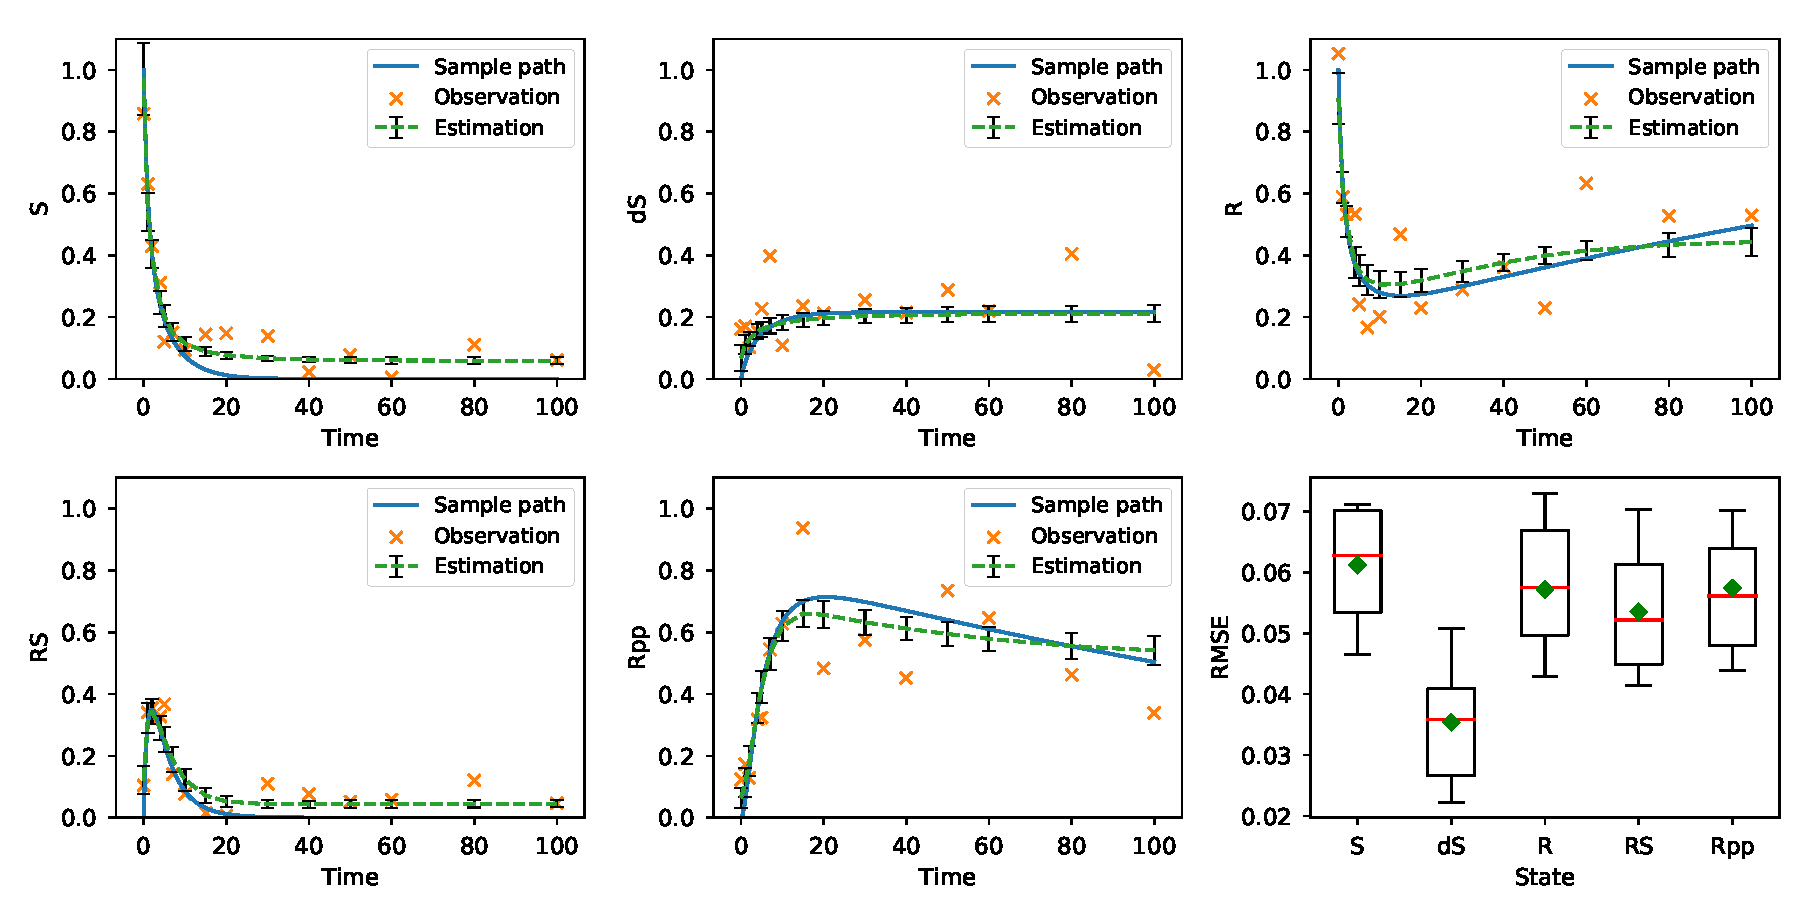
\includegraphics[width=\textwidth]{graphics/protein-states-without-km}
    \caption{State estimation results for the protein signaling transduction pathway model with the parameter $K_m$ set to constant. The ground truth is shown as the blue line. The observations, when available, are shown as the orange crosses. The estimation is shown as the dotted green line. The error bars in the first five plots indicate one standard deviation. For the box plot, the median is indicated by the red line, while the mean is shown as the green diamond. The box shows the lower and upper quartiles, while the whiskers are the 5th and 95th percentiles.}
    \label{fig-protein-states-without-km}
\end{figure}

\begin{figure}
    \centering
    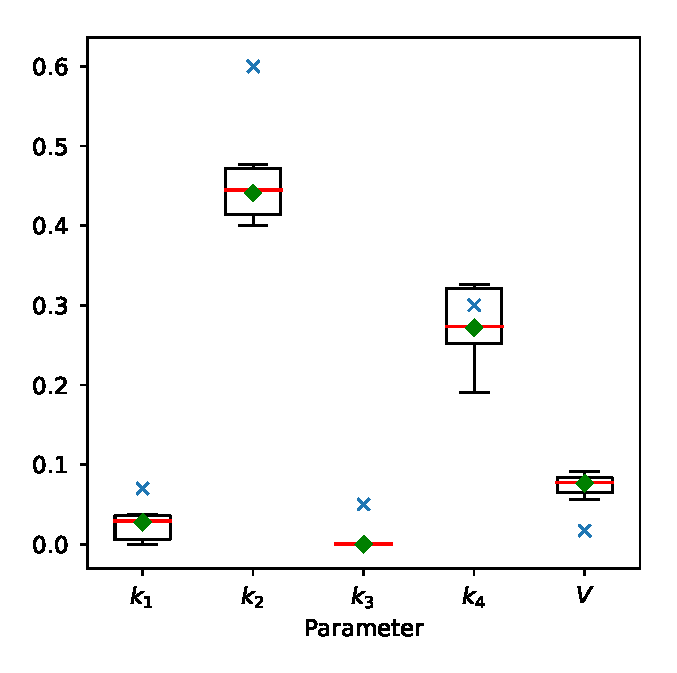
\includegraphics[width=0.48\textwidth]{graphics/protein-parameters-without-km}
    \caption{Parameter estimation results for the protein signaling transduction pathway model with the parameter $K_m$ set to constant. In the box plot, the median is indicated by the red line, while the mean is shown as the green diamond. The box shows the lower and upper quartiles, while the whiskers are the 5th and 95th percentiles. The true parameter values are indicated by the blue crosses.}
    \label{fig-protein-parameters-without-km}
\end{figure}

\begin{figure}
    \centering
    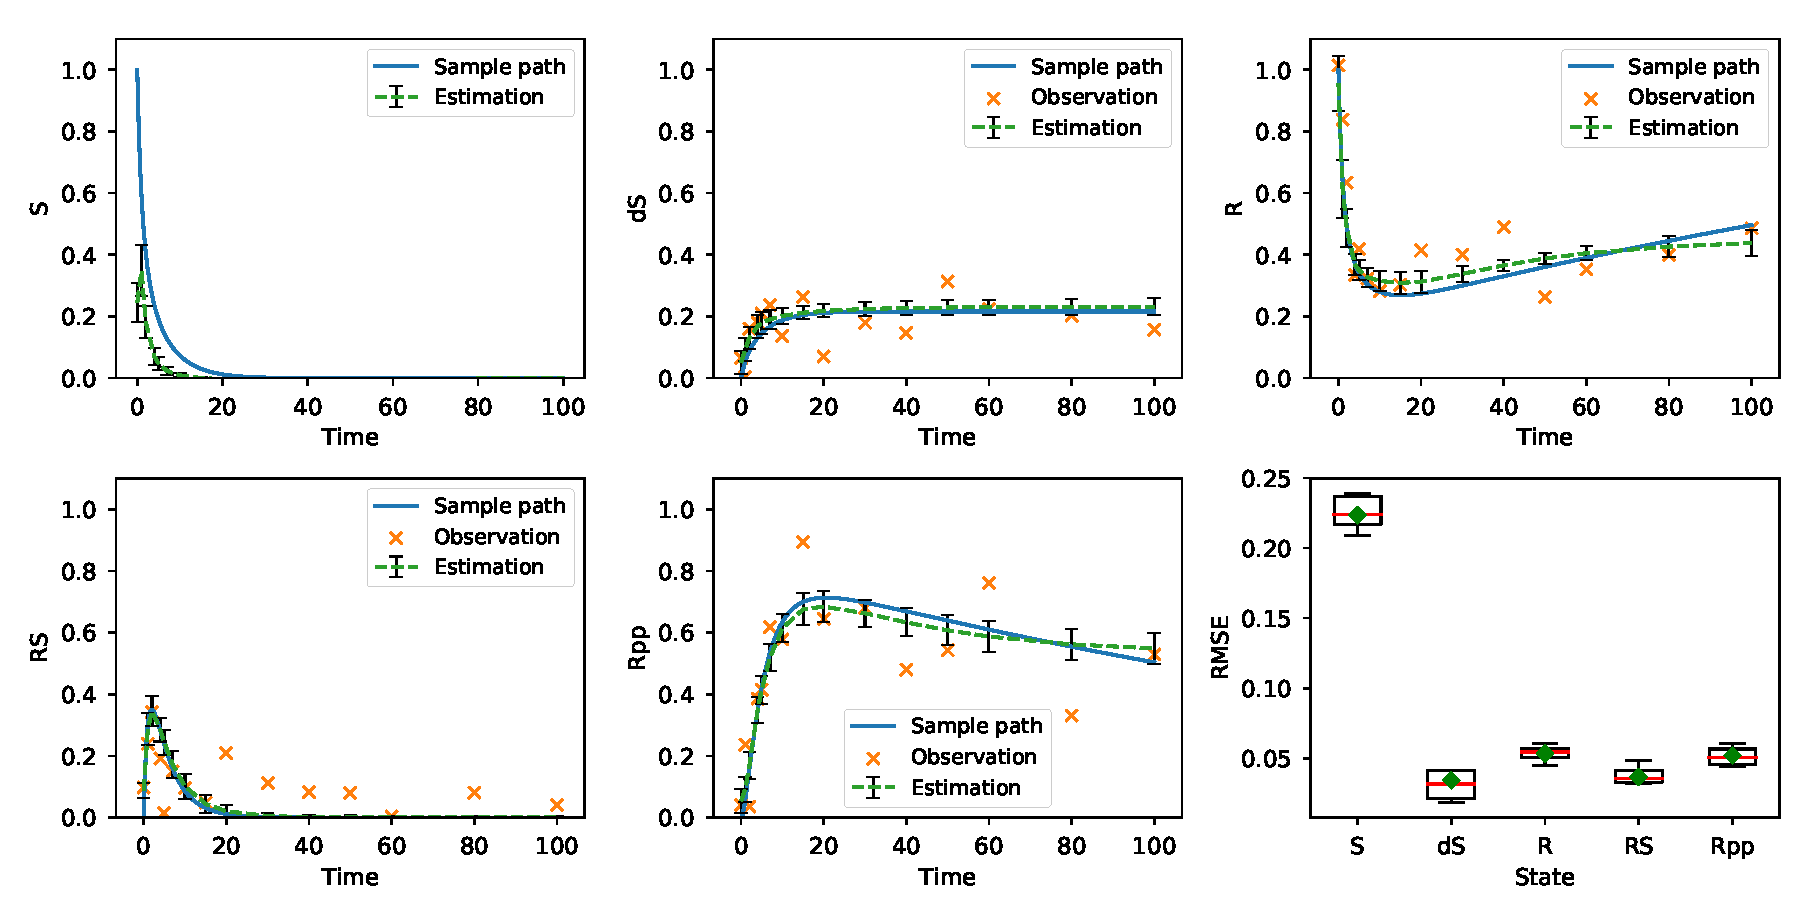
\includegraphics[width=\textwidth]{graphics/protein-states-without-km-partial}
    \caption{State estimation results for the protein signaling transduction pathway model with the parameter $K_m$ set to constant and the state $S$ unobservable. The ground true is shown as the blue line. The observations, when available, are shown as the orange crosses. The estimation is shown as the dotted green line. The error bars in the first five plots indicate one standard deviation. For the box plot, the median is indicated by the red line, while the mean is shown as the green diamond. The box shows the lower and upper quartiles, while the whiskers are the 5th and 95th percentiles.}
    \label{fig-protein-states-partial-without-km}
\end{figure}

\begin{figure}
    \centering
    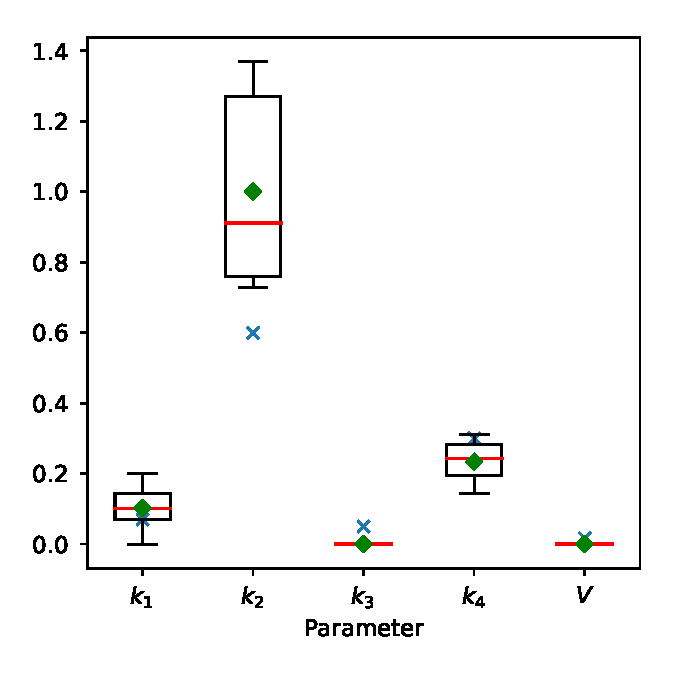
\includegraphics[width=0.48\textwidth]{graphics/protein-parameters-without-km-partial}
    \caption{Parameter estimation results for the protein signaling transduction pathway model with the parameter $K_m$ set to constant and the state $S$ unobservable. In the box plot, the median is indicated by the red line, while the mean is shown as the green diamond. The box shows the lower and upper quartiles, while the whiskers are the 5th and 95th percentiles. The true parameter values are indicated by the blue crosses.}
    \label{fig-protein-parameters-partial-without-km}
\end{figure}

\subsubsection*{Direct inference on $Rpp$}

In this experiment, the parameter $K_m$ is not inferred but all the states are directly inferred.
This setup includes the $Rpp$ state that violates the structural assumption, which is not possible using the \algovgmgp\ method.
The results after 10 independent repetitions are shown in \reffigure{\ref{fig-protein-states-without-km}} and \reffigure{\ref{fig-protein-parameters-without-km}}.
For state estimation, the overall trend of the states is captured by the learning algorithm.
Since there are much fewer observations toward the end of the time point, the prediction becomes worse.
The parameter estimation result is not ideal in comparison to the states.

\subsubsection*{Partial observation}

To increase the difficult of the problem, the observations on the state $S$ is masked out.
The results after 10 independent repetitions is shown in \reffigure{\ref{fig-protein-states-partial-without-km}} and \reffigure{\ref{fig-protein-parameters-partial-without-km}}.
Given even less observations, the accuracy of both state and parameter estimation become worse.
From \reffigure{\ref{fig-protein-states-partial-without-km}} it can be seen that gradient model indeed does provide some guidance on the estimation of the state $S$.

\section{Lorenz 96 model}
\label{sec-lorenz-96}

As a minimalistic weather forecast model, the \emph{Lorenz 96} model \citep{lorenz1996predictability} is another widely used benchmark system due to its chaotic behavior under certain configurations and its flexibility to scale to large numbers of states.
A $K$-dimensional deterministic Lorenz 96 dynamical system is defined for $k = \mrange{1}{K}$, state-wise as follows:
\begin{align}
    \dymdxktn{k}{}
     & = (\dymxktn{k+1}{} - \dymxktn{k-2}{})\dymxktn{k-1}{} - \dymxktn{k}{} + F
    \label{eq-lorenz-96-drift}
\end{align}
where $\dymxktn{-1}{} = \dymxktn{K-1}{}$, $\dymxktn{0}{} = \dymxktn{K}{}$, $\dymxktn{K+1}{}=\dymxktn{1}{}$, and $F \in \R$ is the parameter controlling the behavior of the system.
When $F < 0.895$, the states decay into a steady value equal to $F$; when $F$ is between 0.895 and 4.0, the states are periodic; when $F \geqslant 4.0$, the system exhibits chaotic behavior \citep{vrettas2015variational}.
An example of the trajectories of a 10-dimensional deterministic Lorenz 96 model is shown in \reffigure{\ref{fig-lorenz-96-trajectories}}.

\begin{figure}
    \centering
    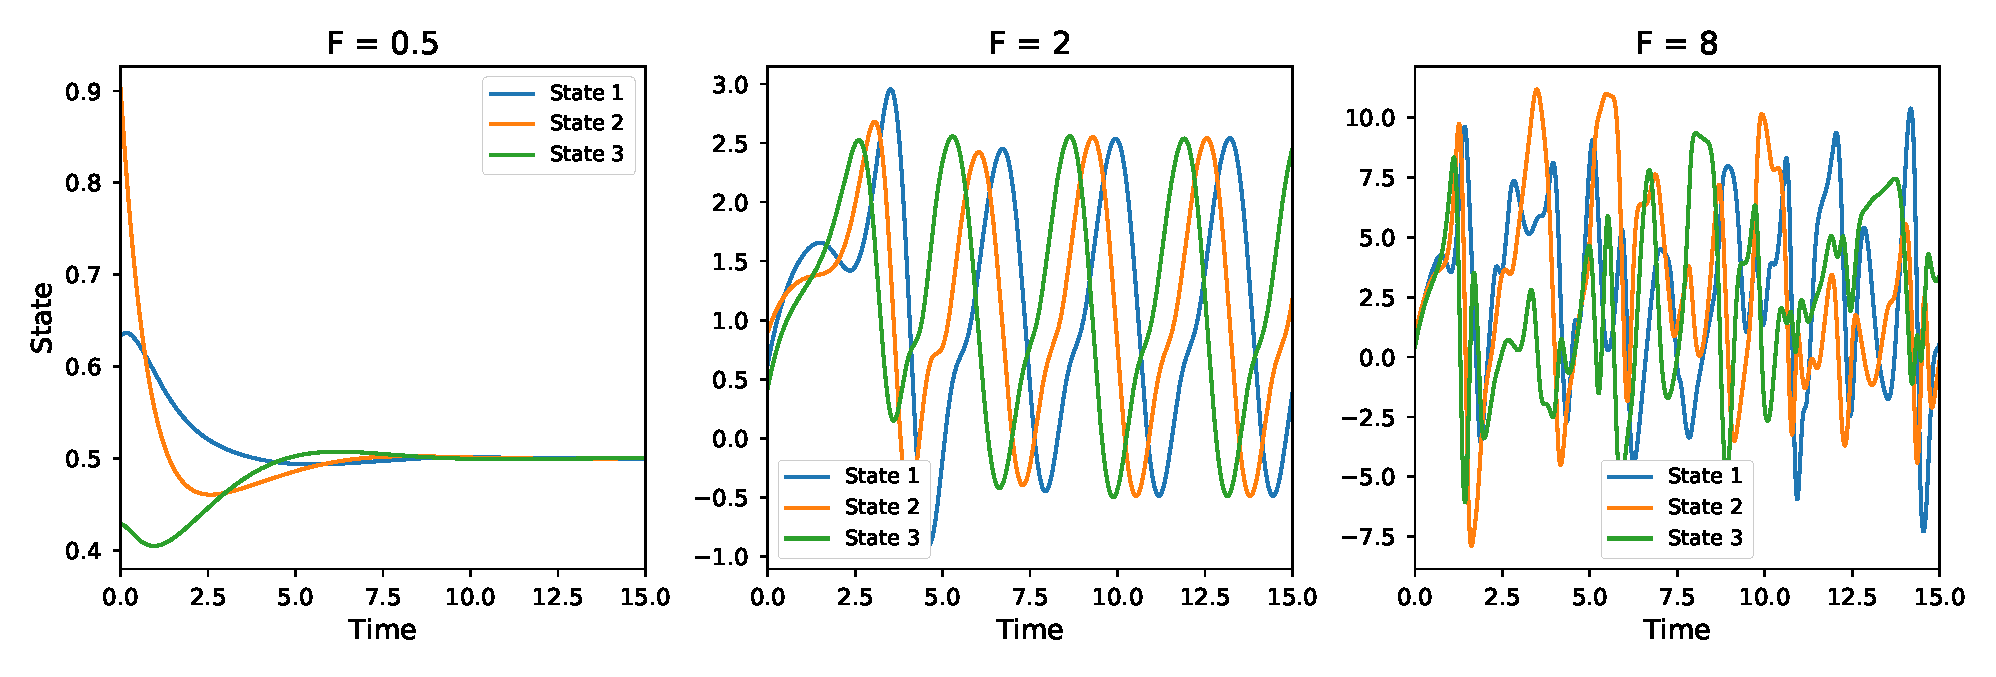
\includegraphics[width=\textwidth]{graphics/lorenz-96-trajectories}
    \caption{Trajectories of the 1st, 2nd and 3rd dimensions of a 10-dimensional deterministic Lorenz 96 model with different parameter values. The numerical integration is carried out from time 0 to 15 with a step size of 0.01.}
    \label{fig-lorenz-96-trajectories}
\end{figure}

The experiments in this section are mainly concerned about the stochastic Lorenz 96 model, which can be obtained by simply including a noise process as described in \refsection{\ref{sec-sdes}}.
Experiments about its deterministic counterpart can be found in \cite{gorbach2017scalable}.
In the following, we compare the results from the \algolpmfsde\ and the \algovgpamf\ methods.

\subsubsection*{Experimental setup}

Following \cite{vrettas2015variational}, \reftable{\ref{table-lorenz-96-setup}} shows the experimental setup to generate sample paths and to collect observations.
The sample paths are generated by the \algovgpamf\ MATLAB code, which uses the first order Euler-Maruyama scheme.
To avoid exploiting the special structure of the drift function \refequationp{\ref{eq-lorenz-96-drift}}, the observed states are selected randomly.
After observations are collected, the data files are converted into the format compatible with the \algolpmfsde\ source code.

\begin{table}
\centering
\caption{Experimental setup to generate sample paths and to collect observations for the stochastic Lorenz 96 model. The system dimension is denoted by $K$ and the number of observable dimensions is $K_{obs}$. Based on the drift parameter $F$ and the diffusion noise, the sample paths are generated from time $t_0$ to $t_T$ with a step size of $\delta t$. The observation noise variance $\dymsigmak{k}^2$ and the diffusion noise variance $\sderhoq{k}^2$ are assumed to be the identical for each state. For each time unit, $freq_{obs}$ denotes the number observations to be collected, which are equally distributed over the time line.}
\label{table-lorenz-96-setup}
\begin{tabular}{|c|c|c|c|c|c|c|c|c|}
\hline
$K$ & $K_{obs}$ & $t_0$ & $t_T$ & $\delta t$ & $F$ & $\dymsigmak{k}^2$  & $\sderhoq{k}^2$ & $freq_{obs}$ \\ \hline
500 & 325 (65\%) & 0 & 4 & 0.01 & 8 & 1 & 4 & 8 \\ \hline
\end{tabular}
\end{table}

Note that the system dimension is scaled down from 1000 to 500 due to time constraints.
Accordingly, the number of observed states is scaled down proportionally.
Nevertheless, it is still very interesting to quantify the scalability of the \algolpmfsde\ solution, which will be examined in detail in a separate experiment later.

For each SDE sample path, the \algolpmfsde\ method averages individual inference results from 100 independently generated RODE sample paths to obtain an ensemble solution.
The RODE sample paths are estimated in parallel on the ETH Euler cluster\footnote{\url{https://scicomp.ethz.ch/wiki/Euler}}.
Only 1 CPU core and 2 GB of memory are allocated to each inference.
For this experiment, the RODE states are estimated using the gradient-based method while the parameters are calculated in closed-form.

On the other hand, the \algovgpamf\ code is deployed on a desktop with an Intel i5 quad-core CPU and 16 GB of memory.
We also note that thread pooling is used to utilize all the CPU resources for the \algovgpamf\ implementation, which is not the case for \algolpmfsde.

\subsubsection*{State estimation}

\begin{figure}
    \centering
    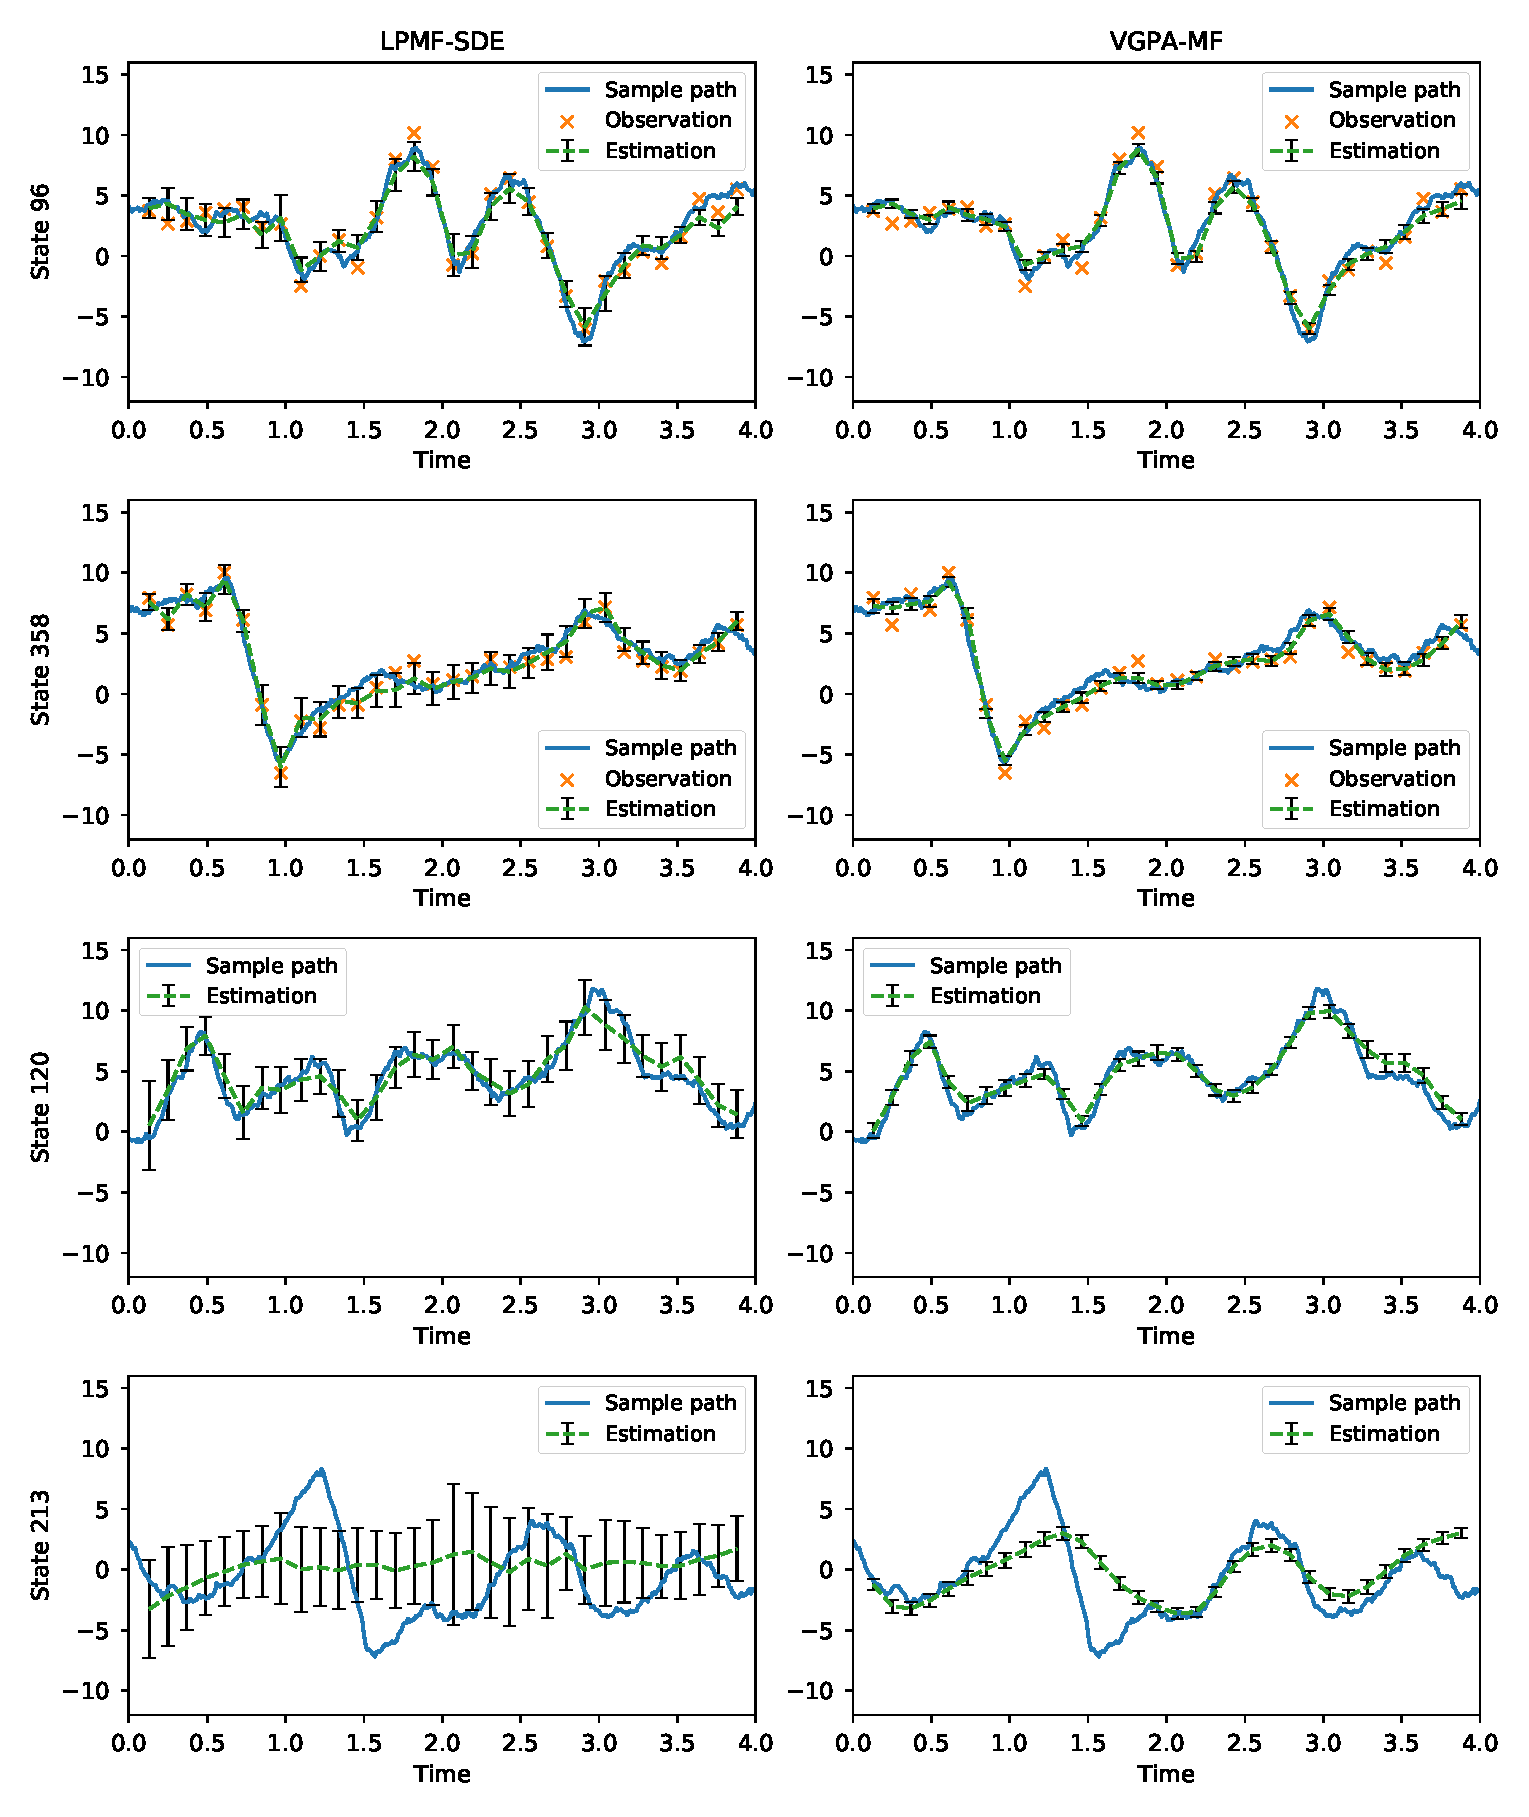
\includegraphics[width=\textwidth]{graphics/lorenz-96-states}
    \caption{State estimation results for 4 selected states from the 500-dimensional stochastic Lorenz 96 model. Among the 500 states, 325 are observed. The left column shows the result using the \algolpmfsde\ method, while the right column contains the result based on the \algovgpamf\ algorithm. In the four rows, state 96 and its neighboring states are directly observed; state 358 and only one side of its neighbors are directly observed; state 120 is not observed but its neighbors are;  state 213 and its neighbors are all unobserved. The ground truth is shown as a solid blue line. The mean of estimation is drawn as a dotted green line together with the error bars indicating one standard deviation. Observations, when available, are indicated by the orange crosses.}
    \label{fig-lorenz-96-states}
\end{figure}

\reffigure{\ref{fig-lorenz-96-states}} shows an example of the state inference result for the stochastic Lorenz 96 model using both methods.
For observed states, the mean values of the predictions from both methods are very close to the ground truth, while the \algovgpamf\ method tends to have lower variance.
For unobserved states, the accuracy of both methods depends on the amount of available information that is directly related to them.
As indicated by the drift function \refequationp{\ref{eq-lorenz-96-drift}}, the states are only coupled with their  neighbors for the Lorenz 96 model.
Therefore, estimation on an unobserved state can be reasonably good when its neighbors are observed, e.g.\ state 120 has observed neighbors 121, 122, 123, etc.
Estimation can fail when the neighbors of that state are also unobserved so that they are unable to provide sufficient information to the algorithm, e.g.\ the true trajectory of state 213 cannot be recovered since states 211 to 215 are all unobserved.
As expected, the uncertainty about the estimation for unobserved states is higher than that for the observed states, which is indicated by the wider error bars.

In order to better quantify the difference between both methods, 10 independent Lorenz 96 SDE sample paths are generated. 
For each SDE sample path, a set of observations is collected, and then the above experiment is repeated.
The root mean square error (RMSE) is used as the accuracy measure, and the RMSEs for observed and unobserved states are considered separately.
The formulas for the RMSEs are
\begin{align}
    RMSE_{obs} 
    & = \frac{1}{K_{obs}}\sum_{k\in \mathcal{S}_{obs}}{\sqrt{
        \frac{1}{N}\sum_{n=1}^N{
            (\dymxhatktn{k}{n} - \dymxktn{k}{n})^2
        }
    }}
    \\
    RMSE_{unobs} 
    & = \frac{1}{K_{unobs}}\sum_{k\in \mathcal{S}_{unobs}}{\sqrt{
        \frac{1}{N}\sum_{n=1}^N{
            (\dymxhatktn{k}{n}-\dymxktn{k}{n})^2
        }
    }}    
\end{align}
where $K_{obs}$ and $K_{unobs}$ indicate the number of observed and unobserved states respectively with $\mathcal{S}_{obs}$ and $\mathcal{S}_{obs}$ as the corresponding sets containing the state indices, $N$ is the total number of observations for each dimension, and $\dymxhatktn{k}{n}$ and $\dymxktn{k}{n}$ are the predicted and true values for the $k$-th state at time point $t$ respectively.

\begin{figure}
    \centering
    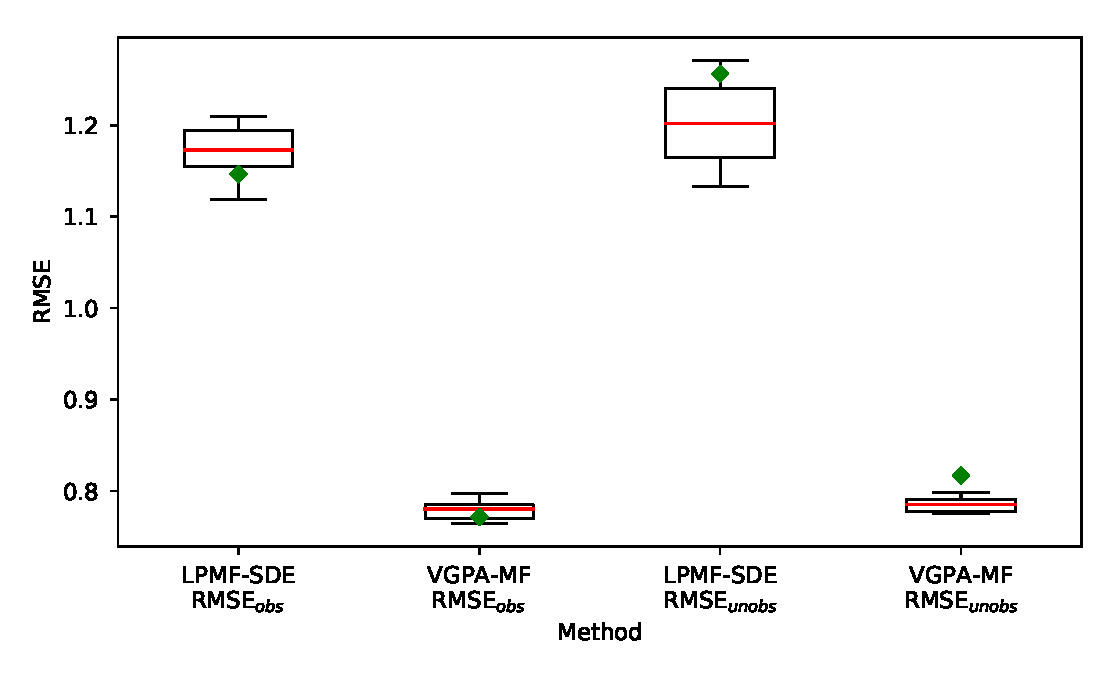
\includegraphics[width=0.8\textwidth]{graphics/lorenz-96-states-boxplot}    
    \caption{Box plot for the RMSEs of state estimation over 10 independent repetitions using sample paths from the 500-dimensional stochastic Lorenz 96 model with 325 observable states. The RMSEs of observed and unobserved states are calculated separately. In the box plot, the median is indicated by the red line, while the mean is shown as the green diamond. The box shows the lower and upper quartiles, while the whiskers are the 5th and 95th percentiles.}
    \label{fig-lorenz-96-state-boxplot}
\end{figure}

The results of the 10 independent repetitions are summarized in \reffigure{\ref{fig-lorenz-96-state-boxplot}}.
At first glance, it is surprising that the \algovgpamf\ method has such low RMSE values.
This is partially because in the MATLAB code we have obtained, only state inference is carried out and the true drift parameter $F$ is given to the inference procedure.
However, the \algolpmfsde\ method is estimating both the states and parameters simultaneously.
Note that the \algovgpamf\ solution is fully capable of jointly estimating the states and parameters.
But as at the time of this writing, we have not obtained the code that computes the gradient of their variational free energy function w.r.t.\ the parameters in order to complete the required experiments.
Moreover, as claimed by \cite{vrettas2015variational}, their  solution can also estimate the diffusion noise, which is an advantage over the \algolpmfsde\ method and can be considered as a possible future extension to this work.
Considering the sparsity of the observations and that the observation noise variances are set to 1, we see some potential for the \algolpmfsde\ solution.

One shortcoming of the \algolpmfsde\ method in this experiment is that it only considers a single optimal value of the cost function found using gradient-based method when making predictions.
Depending on the initialization conditions and the complexity of the cost function, which is subject to the complexity of drift function, sometimes the optimization procedure can be trapped in a local optimum.
As a consequence, even though the mean is  recovered reasonably well, the variance of the prediction is less under control.
Since currently only out-of-package second-order optimization techniques such as the \emph{truncated Newton method}, the \emph{dog-leg trust-region algorithm}, etc. \citep{nocedal2006numerical}, are used, further improvement on the optimization strategy can also be considered as an extension to this work.

\subsubsection*{Parameter estimation}

This section only discusses parameter inference results. 
Using the \algolpmfsde\ algorithm, the result for a single SDE sample path is illustrated in \reffigure{\ref{fig-lorenz-96-parameters}}, while the result from the 10 dependent repetitions is summarized in \reffigure{\ref{fig-lorenz-96-parameters-boxplot}}.
Due to the lack of relevant files from the \algovgpamf\ MATLAB code as mentioned previously, grid search with a step size of 0.5 is performed on one sample path and result is shown in \reffigure{\ref{fig-lorenz-96-parameters-grid-search}}.

\begin{figure}
    \centering
    \begin{subfigure}[b]{0.48\textwidth}
        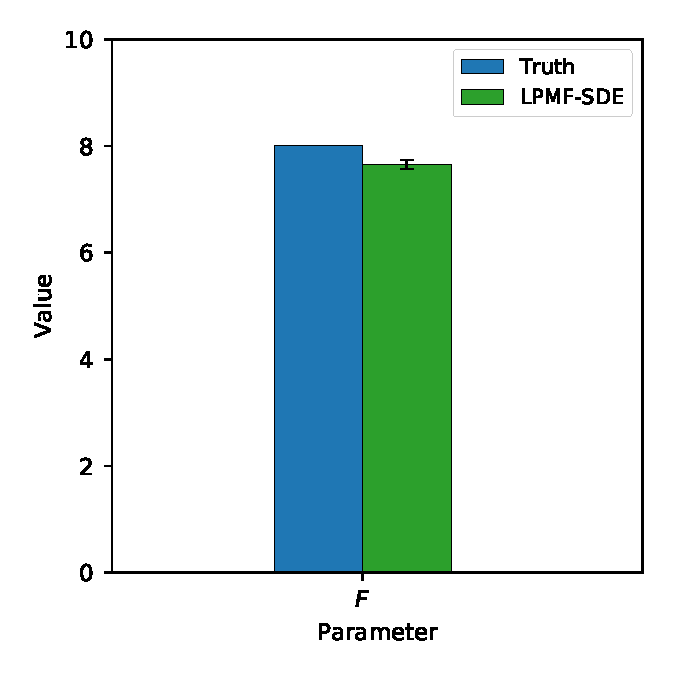
\includegraphics[width=\linewidth]{graphics/lorenz-96-parameters}
        \caption{\ }
        \label{fig-lorenz-96-parameters}
    \end{subfigure}
    \begin{subfigure}[b]{0.48\textwidth}
        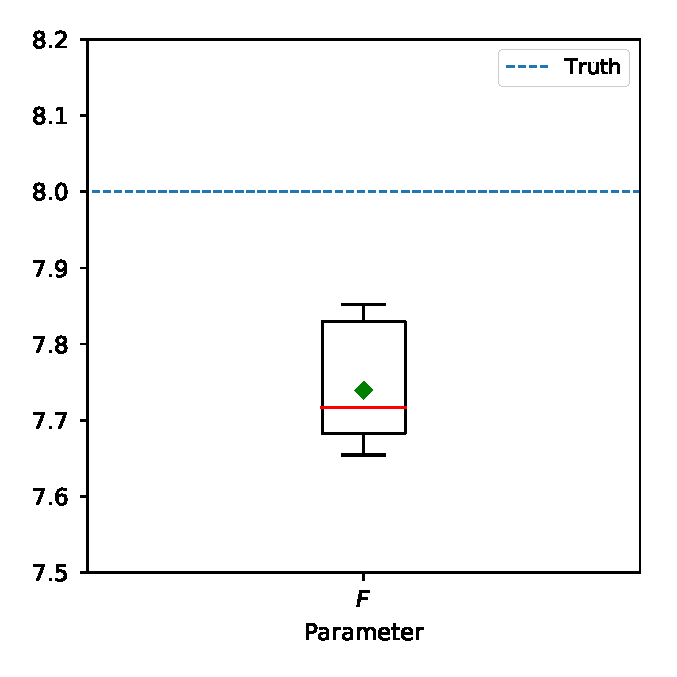
\includegraphics[width=\linewidth]{graphics/lorenz-96-parameters-boxplot}
        \caption{\ }
        \label{fig-lorenz-96-parameters-boxplot}
    \end{subfigure}
    \caption{Parameter estimation result using the \algolpmfsde\ algorithm for the 500-dimensional stochastic Lorenz 96 model with 325 observable states. (a) Estimation result for the SDE sample path shown in \reffigure{\ref{fig-lorenz-96-states}}. The blue bar indicates the true parameter value. The green bar shows the mean of estimation by averaging individual results from 100 RODE sample paths. The error bar indicates one standard deviation. (b) Box plots for parameter estimation over 10 independent repetitions. In the box plot, the median is indicated by the red line, while the mean is shown as the green diamond. The box shows the lower and upper quartiles, while the whiskers are the 5th and 95th percentiles. The dotted blue line indicates the true parameter value.}
    \label{fig-lorenz-96-parameters-group}    
\end{figure}

\begin{figure}
    \centering
    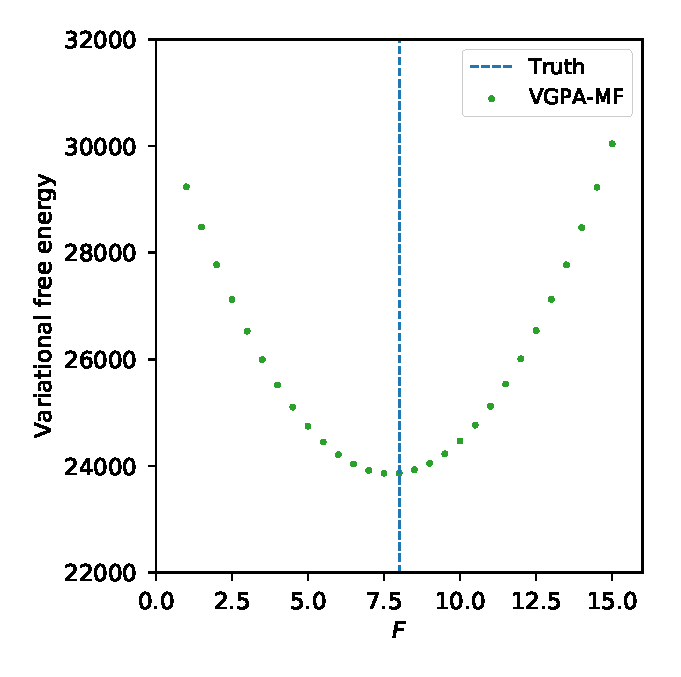
\includegraphics[width=0.48\textwidth]{graphics/lorenz-96-parameters-grid-search}
    \caption{Grid search result using the \algovgpamf\ algorithm for the stochastic Lorenz 96 model using sample paths shown in \reffigure{\ref{fig-lorenz-96-states}}. The green dots indicate where the grid search is carried out, while the dash blue line indicates the true parameter value.}        
    \label{fig-lorenz-96-parameters-grid-search}
\end{figure}

\reffigure{\ref{fig-lorenz-96-parameters}} shows that the estimation of the drift parameter $F$ is very close to the true value 8, and the variance is much lower in comparison to state estimation.
This is due to the fact that the Lorenz 96 model has only one drift parameter, which appears inside the drift function for each state.
Hence, the gradient matching model is able to obtain much more information about the drift parameter, despite the existence of unobserved states.
\reffigure{\ref{fig-lorenz-96-parameters-boxplot}} further shows that the mean values of parameter estimation over the 10 independent repetitions are narrowly distributed.
But in general, the \algolpmfsde\ method tends to underestimate the parameter value.
Lastly, although \reffigure{\ref{fig-lorenz-96-parameters-grid-search}} shows that the variational free energy of the \algovgpamf\ algorithm reaches the minimum at the true parameter value, but the whole experiment took almost 36 hours to complete.
For dynamical system with several parameters, the combinatorial nature of the parameters would render this approach impractical.

\subsubsection*{Runtime performance}

For the SDE sample path shown in \reffigure{\ref{fig-lorenz-96-states}}, the average runtime for the \algolpmfsde\ algorithm to solve one RODE sample path is 2309 seconds with a standard deviation of around 128 seconds, while the runtime for the \algovgpamf\ method takes 3232 seconds.
As the current \algovgpamf\ MATLAB code only runs the state smoothing algorithm, it is expected to be much more computationally intensive when parameter estimation is carried out simultaneously, since the forward-backward loop has to be entered many times until convergence.

\begin{figure}
    \centering
    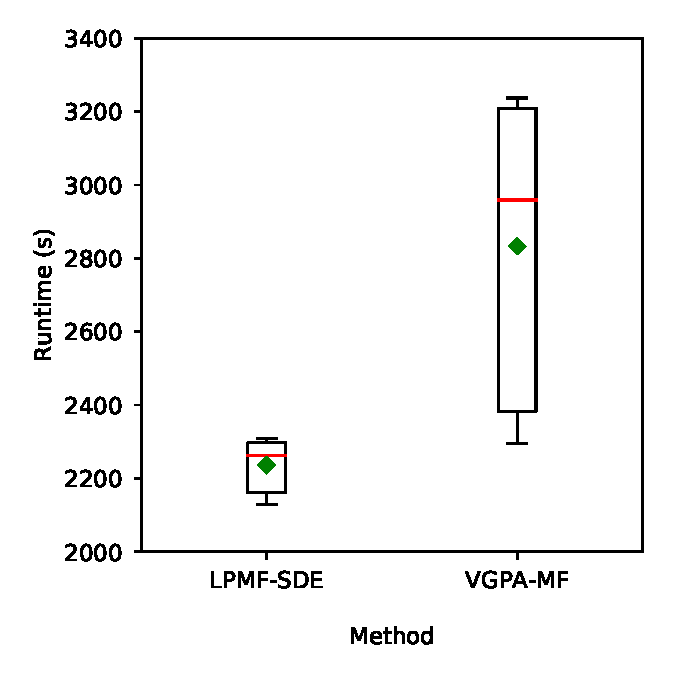
\includegraphics[width=0.48\textwidth]{graphics/lorenz-96-runtime-boxplot}
    \caption{Box plot for the runtimes over 10 repetitions using independent sample paths from the stochastic Lorenz 96 model. The median is indicated by the red line, while the mean is shown as the green diamond. The box shows the lower and upper quartiles, while the whiskers are the 5th and 95th percentiles.}        
    \label{fig-lorenz-96-runtime-boxplot}
\end{figure}

\reffigure{\ref{fig-lorenz-96-runtime-boxplot}} summarizes the average runtimes for \algolpmf\ to solve one RODE sample path and the runtimes for \algovgpamf\ to complete one iteration of state smoothing over the 10 independent repetitions.
It shows that the \algolpmfsde\ solution performs consistently faster and more stably than its counterpart, as indicated by lower median runtime value and the narrower distribution.

To conclude, the \algolpmfsde\ algorithm requires much less resources and also runs faster for inference on one RODE sample path.
However, the ensemble nature of the \algolpmfsde\ strategy relies on averaging results from a large number RODE estimations, which could increase the computational requirements significantly.
Nevertheless, given the availability of computer farms and the ease of setting up distributed inference pipeline nowadays, the parallelism requirement for the \algolpmfsde\ solution can be easily satisfied. 


\subsubsection*{Scalability}

\begin{figure}
    \centering
    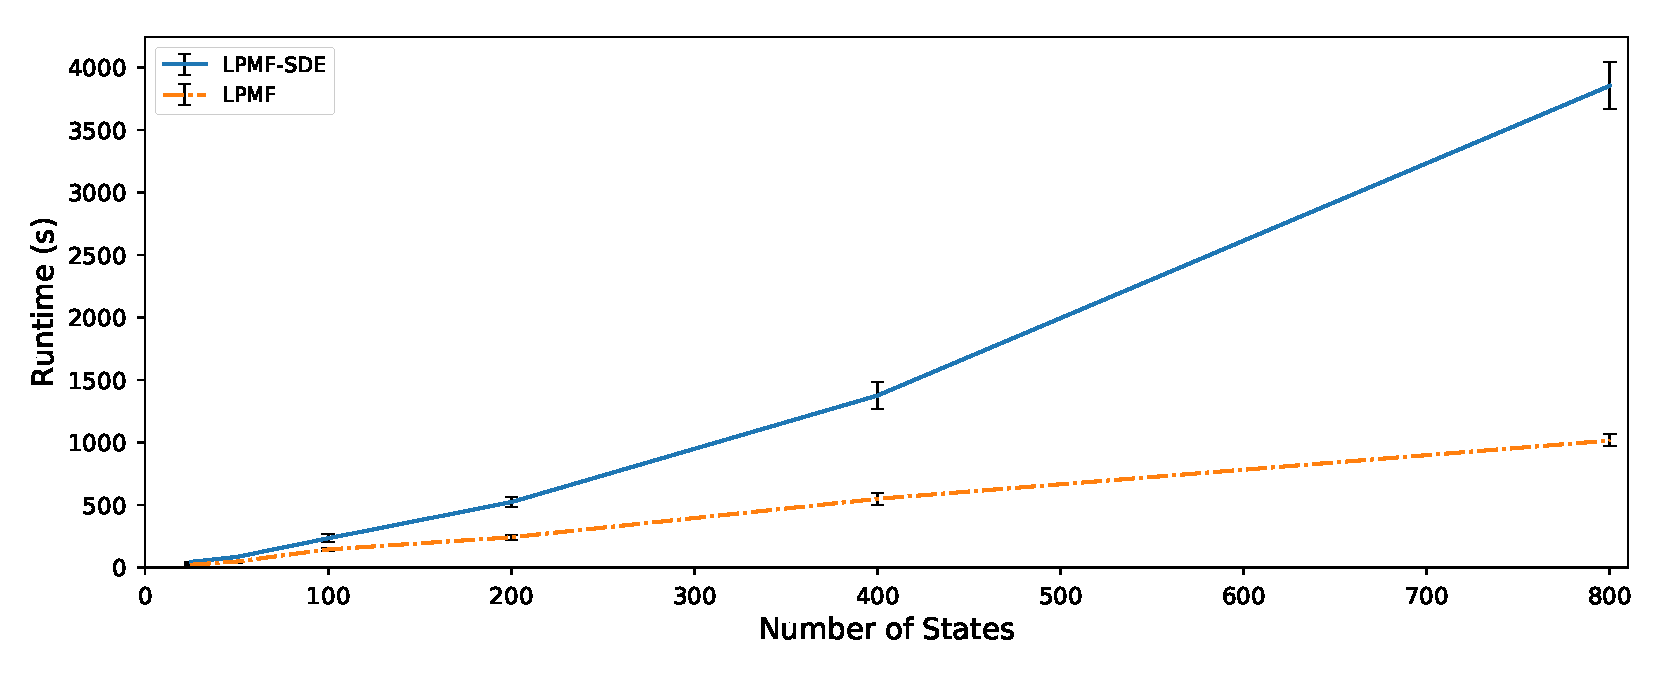
\includegraphics[width=\textwidth]{graphics/lorenz-96-scalability}
    \caption{Scalability of the \algolpmfsde\ algorithm versus its deterministic counterpart, i.e.\ \algolpmf, as the dimensionality of the system increases. For the \algolpmfsde\ method, the blue line indicates the average interpolated runtime to inference one RODE sample path over 10 independent RODE sample paths by connecting the measurements at 25, 50, 100, 200, 400 and 800. For the \algolpmf\ method, the orange line is obtained by connecting the averages of 10 independent runs on the same ODE trajectory with different observations at the same measurement points. The error bars in both setups indicate one standard deviation.}
    \label{fig-lorenz-96-scalability}
\end{figure}

As mentioned by \cite{gorbach2017scalable}, inference on the deterministic Lorenz 96 model with 1000 states using their \algovgmgp\ solution completes within 400 seconds on average.
However, the \algolpmfsde\ method, which extends their methodology, takes on average more than 2200 seconds for one RODE sample path with only 500 states, as shown in \reffigure{\ref{fig-lorenz-96-runtime-boxplot}}.
It is therefore interesting to re-examine the scalability of the \algolpmfsde\ solution.

First, we noticed during implementation that the performance of the \algolpmf\ method for ODEs is comparable to the \algovgmgp\ method.
The major difference between \algolpmfsde\ and \algolpmf\ is the introduction of a stochastic Ornstein-Uhlenbeck process into the vector field of the ODEs.
To reveal the influence of the stochastic process on the inference procedure, the following experiment compares side-by-side the performance of the \algolpmfsde\ method running on the stochastic Lorenz 96 model with the performance of the \algolpmf\ method running on its deterministic counterpart as the number of states increases.

Specifically, measurements are taken with a system dimensionality of 25, 50, 100, 200, 400, and 800 with the number of observed states kept at 65 percent of the total number of states.
Using the same setup in \reftable{\ref{table-lorenz-96-setup}}, except that the diffusion noise is not used for the Lorenz 96 ODEs, the \algolpmfsde\ algorithm is tested with 10 independent RODE sample paths while the \algolpmf\ method is tested with 10 independent observation sets from the same ODE trajectory for each system dimensionality.
The experiments are all conducted on the Euler cluster with the same hardware configuration.

As can be seen from \reffigure{\ref{fig-lorenz-96-scalability}}, benefiting from the efficient implementation of the gradient and Hessian evaluation subroutines, the gradient-based \algolpmf\ method incurs only a slightly higher performance penalty than the closed-form solution from \algovgmgp.
Also, the runtime seems to increase linearly as the number of states increases.
On the other hand, the performance of the \algolpmfsde\ method degrades much faster than \algolpmf, and the gap between them become larger as the number of states increases.
The cause of this phenomenon requires further investigation but a plausible explanation is the complication of the optimization objective after the introduction of the stochastic process into the vector field.

\vspace{\baselineskip}
\section{Lorenz 63 model}
\label{sec-lorenz-63}

The last dynamical system examined in this chapter is the stochastic version of the \emph{Lorenz 63} model \citep{lorenz1963deterministic}, which is a low dimensional mathematical model for thermal convection in the atmosphere.
The vector field of the deterministic Lorenz 63 is defined as follows:
\begin{align}
    \dymf
    & =
    \begin{bmatrix}
        \dot{x}(t)
        \\ 
        \dot{y}(t)
        \\
        \dot{z}(t)
    \end{bmatrix}
    =
    \begin{bmatrix}
        \sigma(y(t) - x(t))
        \\
        x(t)(\rho - z(t)) - y(t)
        \\
        x(t)y(t) - \beta z(t)
    \end{bmatrix}
    \label{eq-lorenz-63-odes}
\end{align}
where the state vector is given by $\dymx = [x(t), y(t), z(t)]^\top \in \R^3$, and $\dymtheta = [\sigma, \rho, \beta]^\top \in \R^3$ is the parameter vector controlling the system behavior.
Although consisting of only 3 states, this model is highly nonlinear and exhibits chaotic behavior under certain parameter configurations.

Correspondingly, the stochastic Lorenz 63 model with a state-specific, additive noise process is given by
\begin{align}
    \sdedx = \sdef \sdedt + \sdeSigma^\frac{1}{2}\sdedwt
\end{align}
where $\sdef$ is defined in \refequationp{\ref{eq-lorenz-63-odes}}, $\sdeSigma \in \R^{3 \times 3}$ is a diagonal matrix containing the diffusion noise variance, and $\sdewt$ is a 3-dimensional standard Wiener process.
Using the parameter set $[10, 28, \frac{8}{3}]^\top$, which is well-known for its resulting chaotic behavior, a sample path is shown in \reffigure{\ref{fig-lorenz-63-sample-path}}.

\begin{figure}
    \centering
    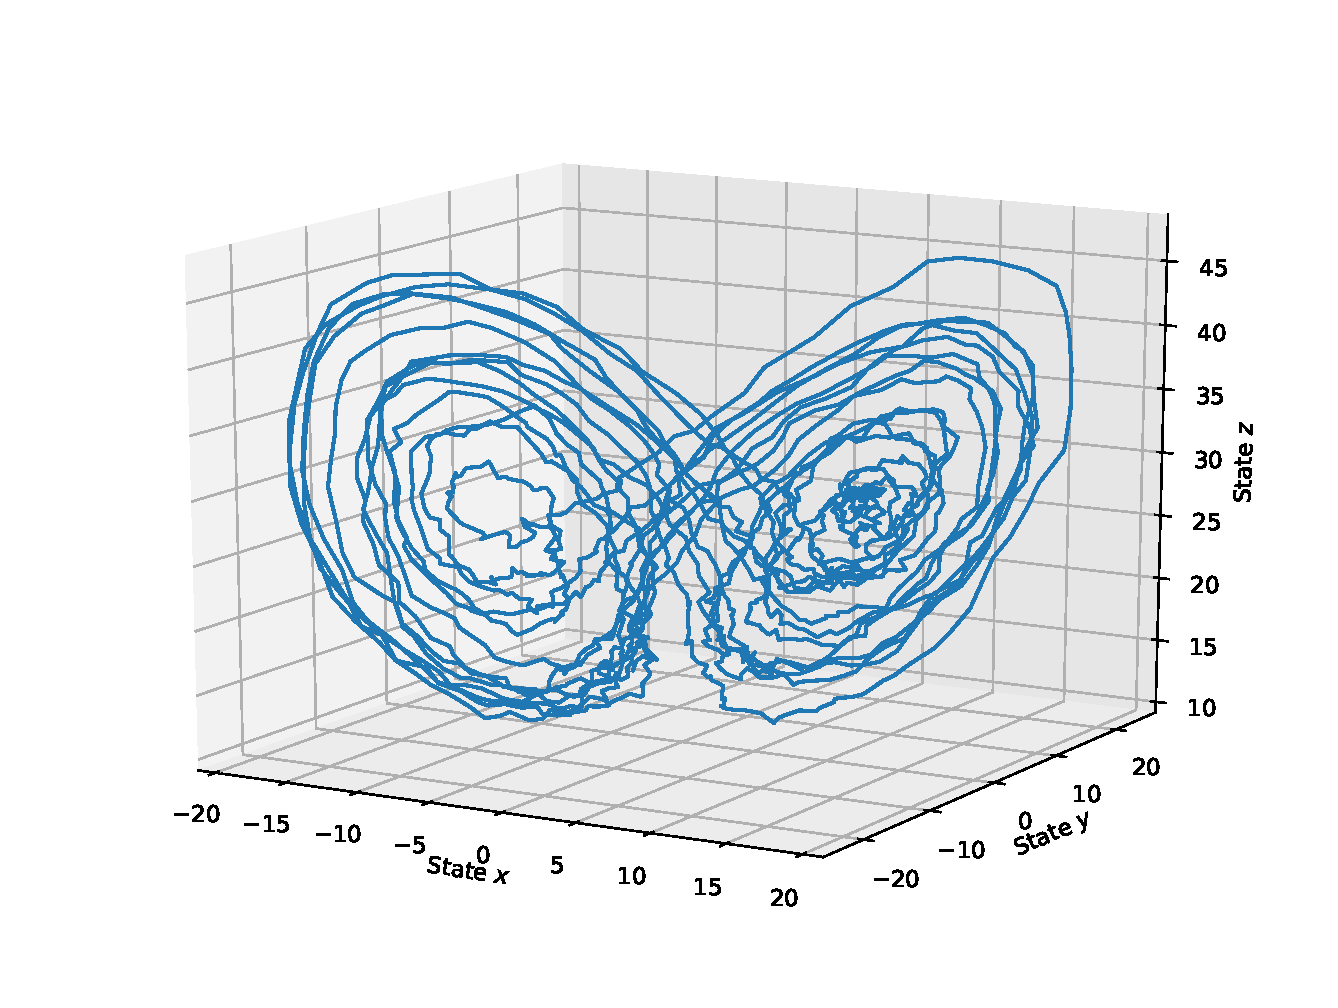
\includegraphics[width=0.8\textwidth]{graphics/lorenz-63-sample-path}
    \caption{Sample path for the stochastic Lorenz 63 model generated based on the parameter values $[\sigma, \rho, \beta]^\top = [10, 28, \frac{8}{3}]^\top$ and the diffusion noise variances $\sderhoq{1}^2 = \sderhoq{2}^2 = \sderhoq{3}^2 = 10$. The integration is performed from time 0 to 20 with a step size of 0.01.}
    \label{fig-lorenz-63-sample-path}
\end{figure}

\subsubsection*{Comparison algorithm}

In order to make comparison, a minimalistic MAP estimation of the drift parameters based on \cite[Table 3]{vrettas2011estimating} is self-implemented\footnote{\url{https://github.com/ruiixu23/VGPA}} by extending the Python source code\footnote{\url{https://github.com/vrettasm/VGPA}} for the \algovgpa\ algorithm.
In the following, the abbreviation \algovgpamap\ is used to refer to this extension.

The extension consists of an inner loop and an outer loop.
The inner loop enhances state estimation by running the \algovgpa\ smoothing algorithm to compute the optimal approximate state posterior, based on the current estimation of the parameters.
The outer loop then takes a gradient step to update the parameters.
This procedure is repeated until either the gradient over the parameters vanishes or the state estimation from the inner loop does not improve further significantly. 
Details of the algorithm can be found in \cite[Section 5.2]{vrettas2011estimating}.

Note that \cite{vrettas2011estimating} claim that the aforementioned algorithm can be similarly applied to the estimation of the diffusion noise covariance matrix $\sdeSigma$, which is not implemented here as the current \algolpmfsde\ method only supports inference on the drift parameters.
Also, the extension adopts a simple gradient update strategy with a fixed learning rate, which may lead to suboptimal result but can nonetheless be used as a baseline.

\subsubsection*{Experimental setup}

Adopting the experimental setup from \cite{vrettas2015variational}, the configuration used to generate sample paths and to collect observations is shown in \reftable{\ref{table-lorenz-63-setup}}.
Specifically, the sample paths are generated by the \algovgpa\ source code using the first order Euler-Maruyama method with a small step size to achieve higher accuracy.
After observations are collected, the data files are transformed into the format compatible with the \algolpmfsde\ method.

\begin{table}
\centering
\caption{Experimental setup to generate sample paths and to collect observations for the stochastic Lorenz 63 model. The system dimension is denoted by $K$ and the number of observable states is denoted by $K_{obs}$. Given the drift parameters $\sigma$, $\rho$, $\beta$ and the diffusion noise, the sample paths are generated from time $t_0$ to $t_T$ with a step size of $\delta t$. The variances of the observation noise $\dymsigmak{k}^2$ and the diffusion noise $\sderhoq{k}^2$ are assumed to be identical for each state. For each time unit, $freq_{obs}$ denotes the number of observations to be collected, which are equally distributed over the time line.}
\label{table-lorenz-63-setup}
\begin{tabular}{|c|c|c|c|c|c|c|c|c|}
\hline
$K$ & $K_{obs}$ & $t_0$ & $t_T$ & $\delta t$ & $\sigma, \rho, \beta$ & $\dymsigmak{k}^2$  & $\sderhoq{k}^2$ & $freq_{obs}$ \\ \hline
3 & 3 or 2 & 0 & 20 & 0.01 & $10, 28, \frac{8}{3}$ & 2 & 10 & 5 \\ \hline
\end{tabular}
\end{table}

In order to provide a fair comparison, both methods are deployed to the Euler cluster using the same hardware configuration described in \refsection{\ref{sec-lorenz-96}}.
For \algolpmfsde, 100 independent RODE sample paths are solved to obtain an ensemble result for one SDE sample path.
The states are optimized using a gradient-based method while the parameters are calculated analytically with mirroring of negative parameters\footnote{The mirroring of negative parameters is a heuristic solution. A better approach would be the enforcement of positivity constraint.}.
For \algovgpamap, the learning rate is fixed to 0.001, the maximum number of iterations is 250, and the stopping criteria are the decrease in the total variational free energy and the \emph{L2 norm} of the change to the drift parameters with a threshold of $10^{-6}$.
We noticed that all the experiments from \algovgpamap\  reached the maximum number of 250 iterations.
After manual examination, the result at the 80th iteration is used for the following comparisons.

It would be interesting to compare these two methods with one unobserved state.
Unfortunately, the smoothing result from the \algovgpa\ algorithm with unobserved state is not ideal from preliminary examination.
Therefore, a comparison with full state observability is provided.
But in order to demonstrate that the \algolpmfsde\ solution is capable of handling partial observations, an additional experiment is conducted by masking out the observations for state $y$.
To distinguish the two scenarios, we use \algolpmfsdef\ and  \algolpmfsdep\ to refer to the fully and partially observable cases respectively.

\begin{figure}
    \centering
    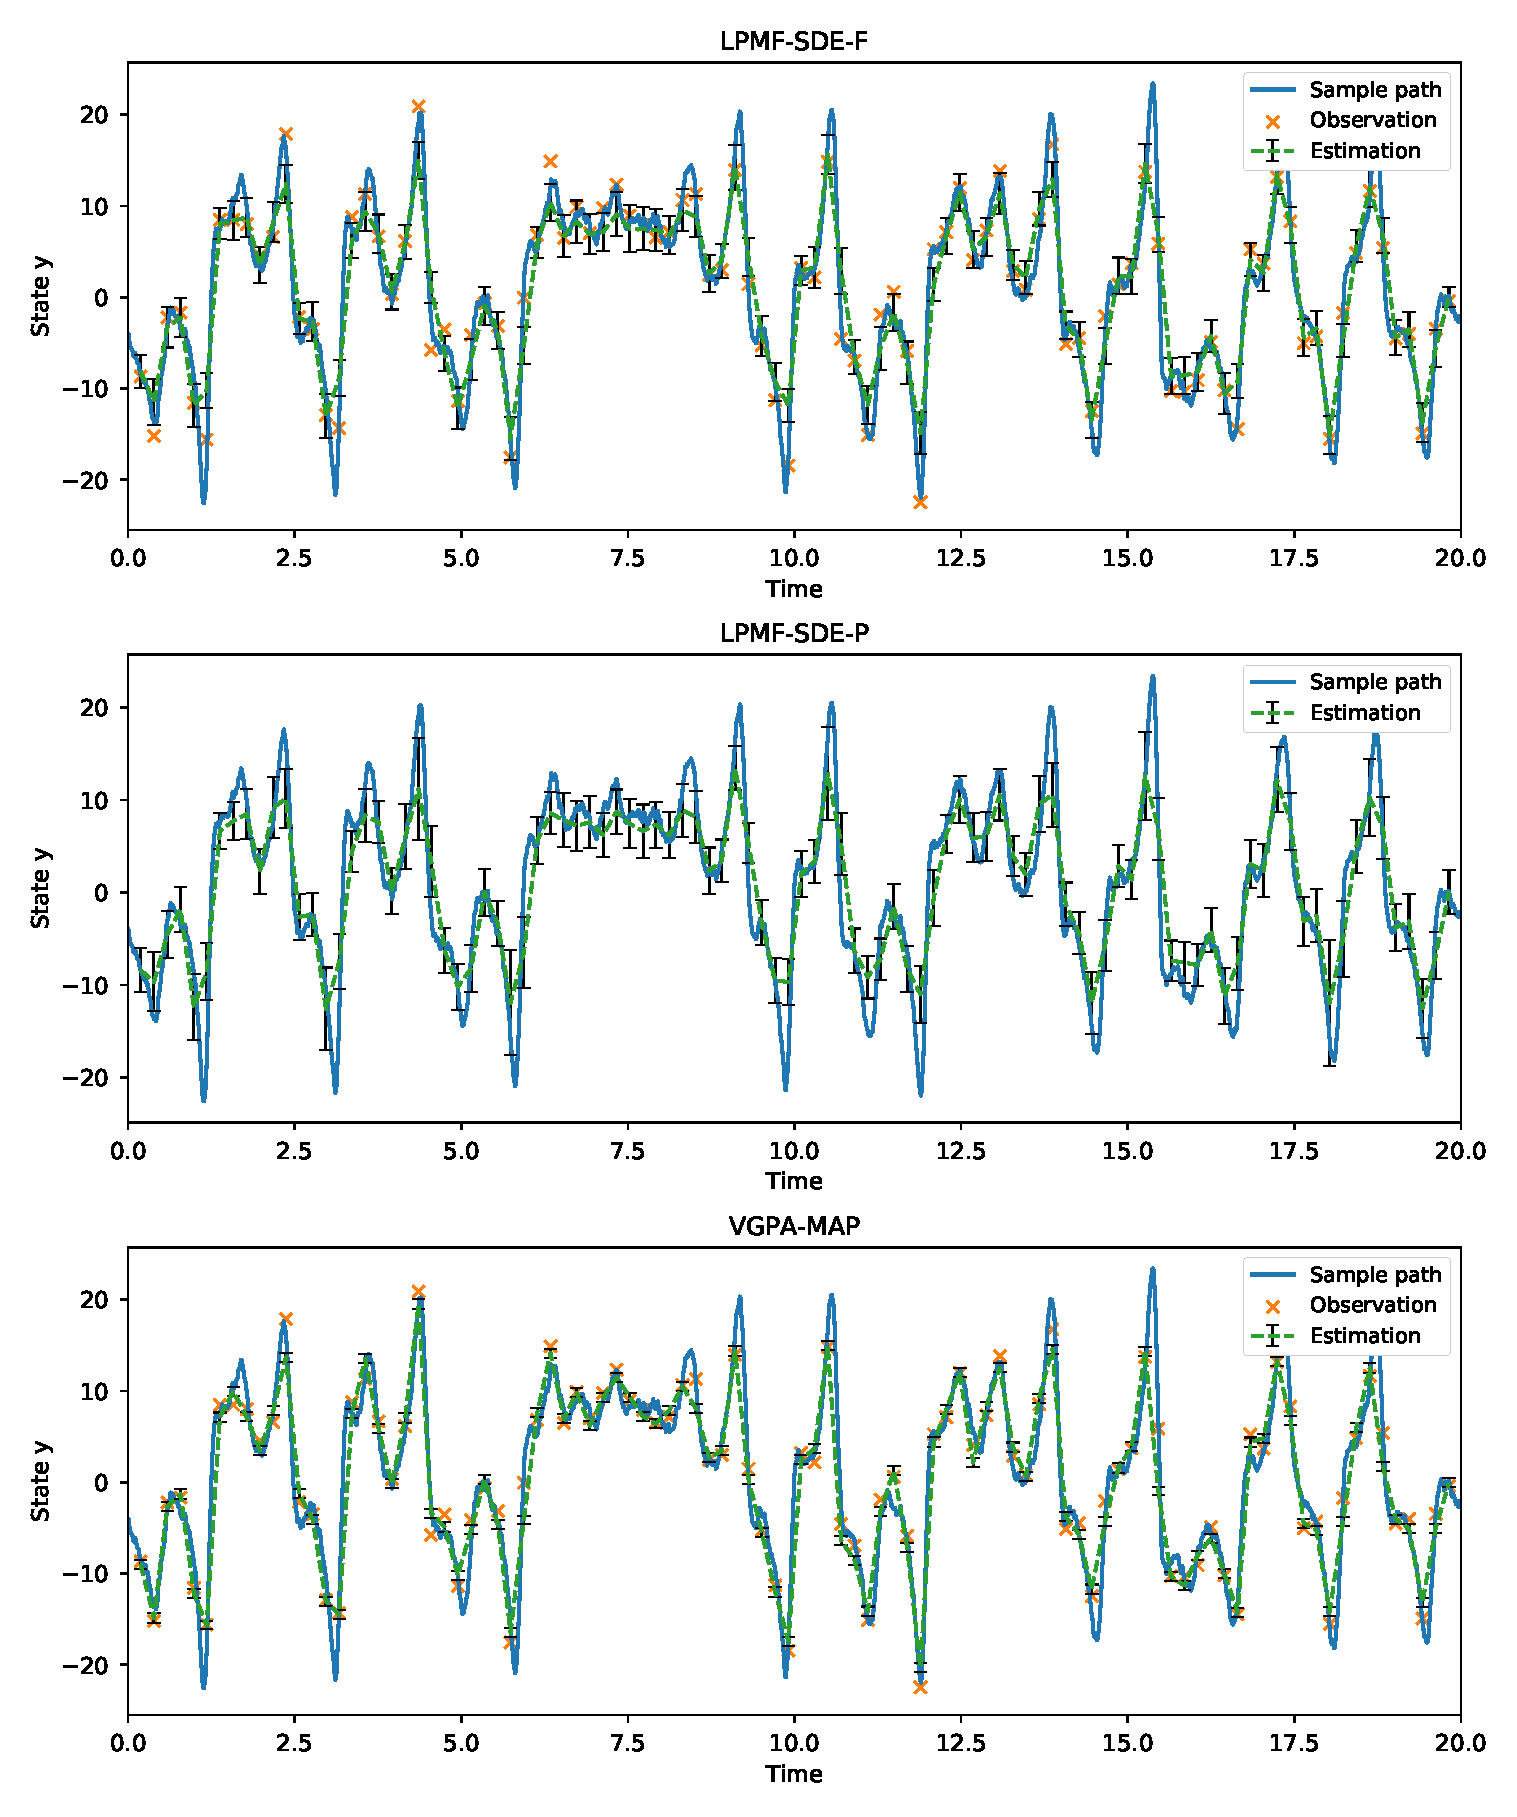
\includegraphics[width=\textwidth]{graphics/lorenz-63-states}
    \caption{Estimation for state $y$ of the stochastic Lorenz 63 model. The top and middle plots are the results for the fully and partially observable cases using the \algolpmfsde\ method respectively. The bottom plot contains the result for the fully observable case using the \algovgpamap\ extension. The ground truth is shown as a solid blue line. The mean of the estimation is drawn as a dotted green line together with the error bars indicating one standard deviation. Observations, when available, are indicated by the orange crosses.}
    \label{fig-lorenz-63-states}
\end{figure}

\begin{figure}
    \centering
    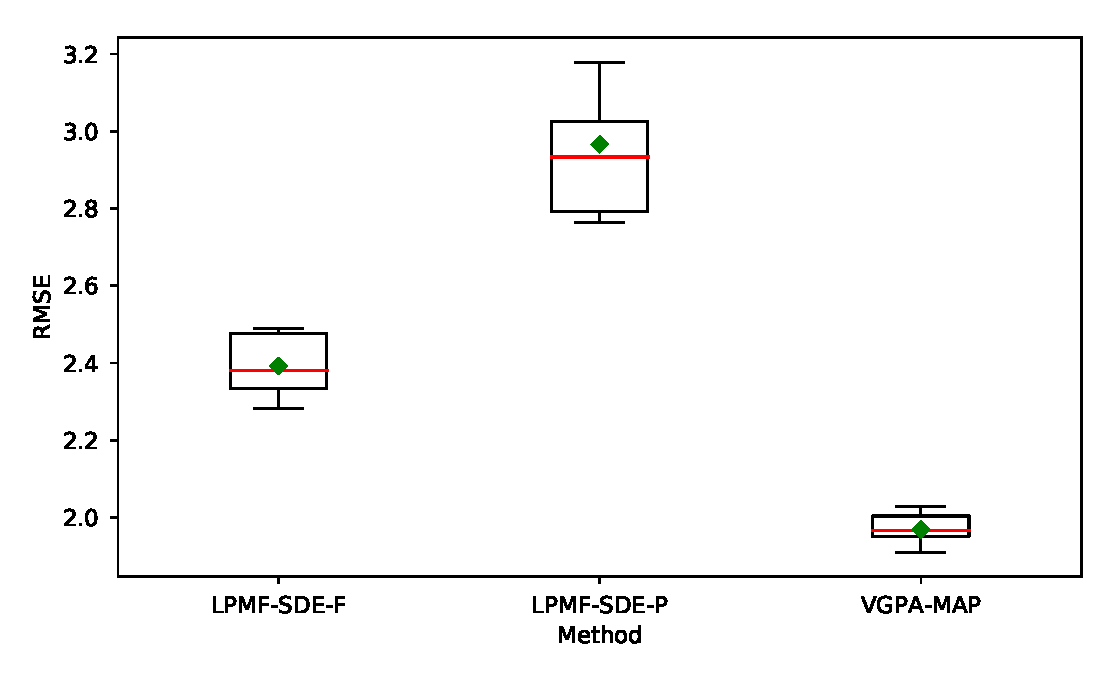
\includegraphics[width=0.8\linewidth]{graphics/lorenz-63-states-boxplot}
    \caption{Box plot for the RMSEs of state estimation over 10 independent SDE sample paths from the stochastic Lorenz 63 model. In the box plot, the median is indicated by the red line, while the mean is shown as the green diamond. The box shows the lower and upper quartiles, while the whiskers are the 5th and 95th percentiles.}
    \label{fig-lorenz-63-state-boxplot}
\end{figure}

\subsubsection*{State estimation}

The estimation for state $y$ from one SDE sample path is shown in \reffigure{\ref{fig-lorenz-63-states}}.
Similar to the result for the stochastic Lorenz 96 model in \refsection{\ref{sec-lorenz-96}}, the general trend of the state is sucessfully captured by both methods with minor differences on the details.
The \algovgpamap\ method seem to be better at points where the state changes dramatically to form high and low peaks.
The variance of the estimation is also lower than the \algolpmfsde\ approach.
One the other hand, it is worth noting that the \algolpmfsde\ method even functions quite well when state $y$ is unobserved but with naturally higher uncertainty, especially around the peaks.
Since state $y$ is unobserved, the only source of information to estimate it is from the drift function \refequationp{\ref{eq-lorenz-63-odes}}, which is demonstrates the potential of the gradient matching framework.

After repeating the above experiment 10 times using each time an independently generated SDE sample path and observation set, the RMSEs for state estimation is computed and summarized in \reffigure{\ref{fig-lorenz-63-state-boxplot}}.
Since there are only three states, the RMSEs over all states are considered together.
The figure shows that the RMSE of state estimation using \algovgpamap\ is slightly below the observation noise variance, which outperforms \algolpmfsde\ with full state observability by around 0.4 on average.
On the other hand, the RMSE using \algolpmfsde\ when state $y$ is unobserved is still reasonably low, considering that the values of the state range from -20 to 20, and the inference is carried out over a much longer time period than all previous experiments.

\subsubsection*{Parameter estimation}

\begin{figure}
    \centering
    \begin{subfigure}{0.48\textwidth}
        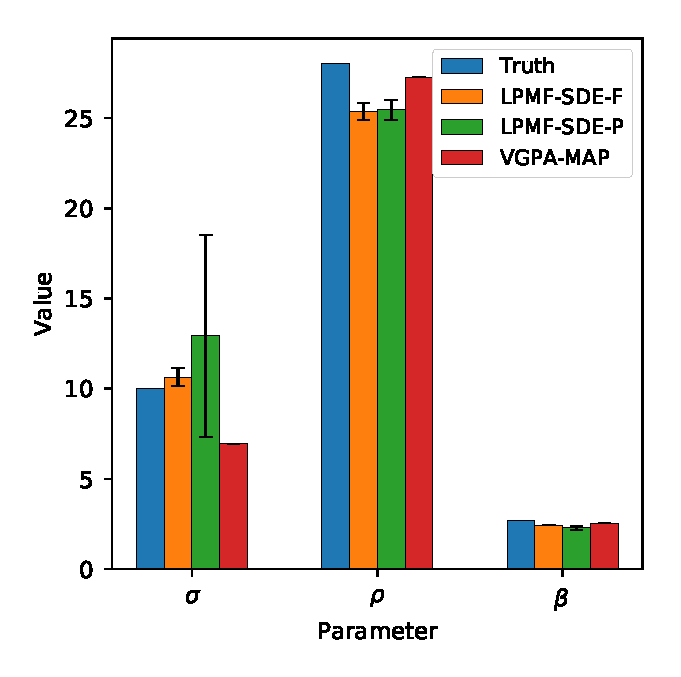
\includegraphics[width=\linewidth]{graphics/lorenz-63-parameters}
        \caption{\ }
        \label{fig-lorenz-63-parameters}
    \end{subfigure}
    \begin{subfigure}{0.48\textwidth}
        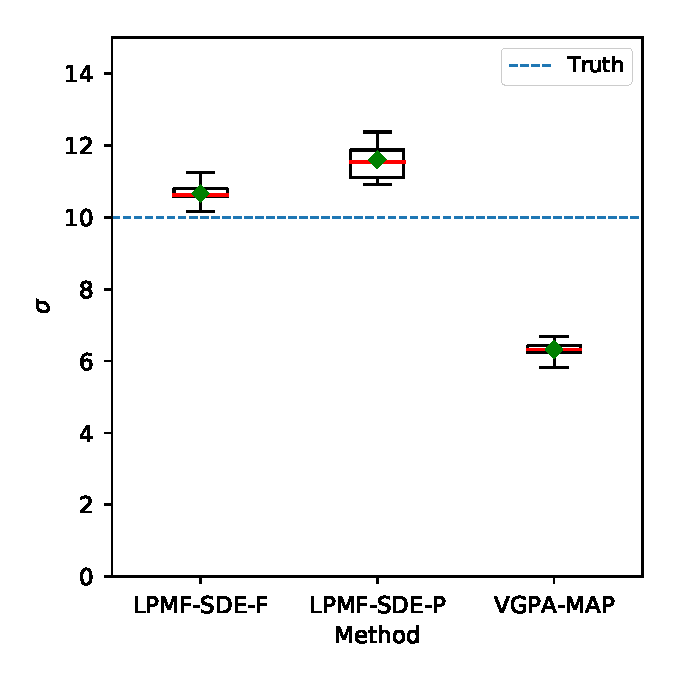
\includegraphics[width=\linewidth]{graphics/lorenz-63-parameters-sigma-boxplot}
        \caption{\ }
        \label{fig-lorenz-63-parameters-sigma-boxplot}
    \end{subfigure}
    \begin{subfigure}{0.48\textwidth}
        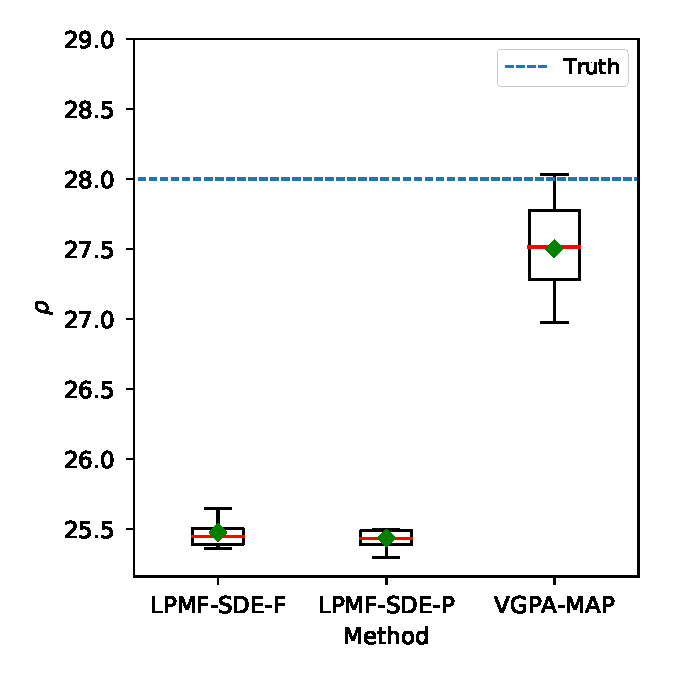
\includegraphics[width=\linewidth]{graphics/lorenz-63-parameters-rho-boxplot}
        \caption{\ }
        \label{fig-lorenz-63-parameters-rho-boxplot}
    \end{subfigure}
    \begin{subfigure}{0.48\textwidth}
        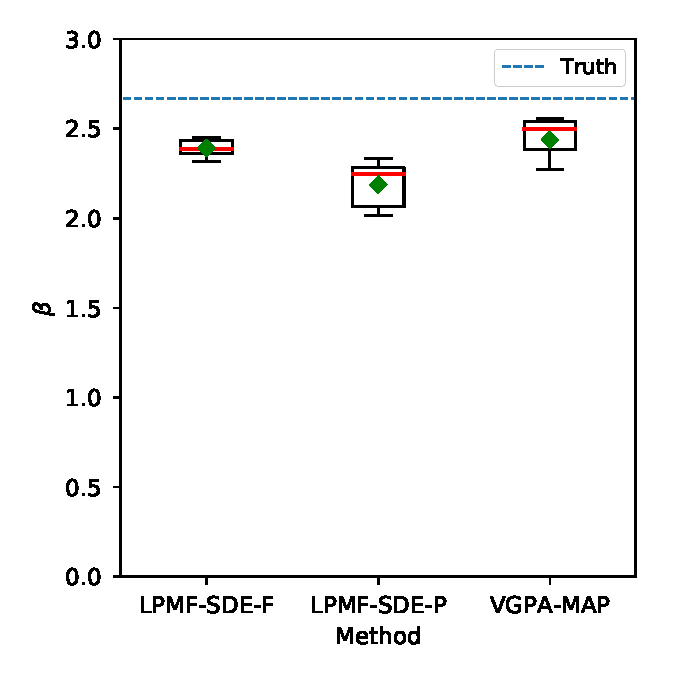
\includegraphics[width=\linewidth]{graphics/lorenz-63-parameters-beta-boxplot}
        \caption{\ }
        \label{fig-lorenz-63-parameters-beta-boxplot}
    \end{subfigure}
    \caption{Parameter estimation result for the stochastic Lorenz 63 model. (a) Estimation result for the SDE sample path shown in \reffigure{\ref{fig-lorenz-63-states}} with the error bar indicating one standard deviation. (b), (c), and (d) are the box plots for parameters $\sigma$,  $\rho$ and $\beta$ after 10 independent repetitions respectively. In the box plot, the median is indicated by the red line, while the mean is shown as the green diamond. The box shows the lower and upper quartiles, while the whiskers are the 5th and 95th percentiles. The dotted blue line indicates the true parameter value.}
    \label{fig-lorenz-63-parameters-group}
\end{figure}

\begin{figure}
    \centering
    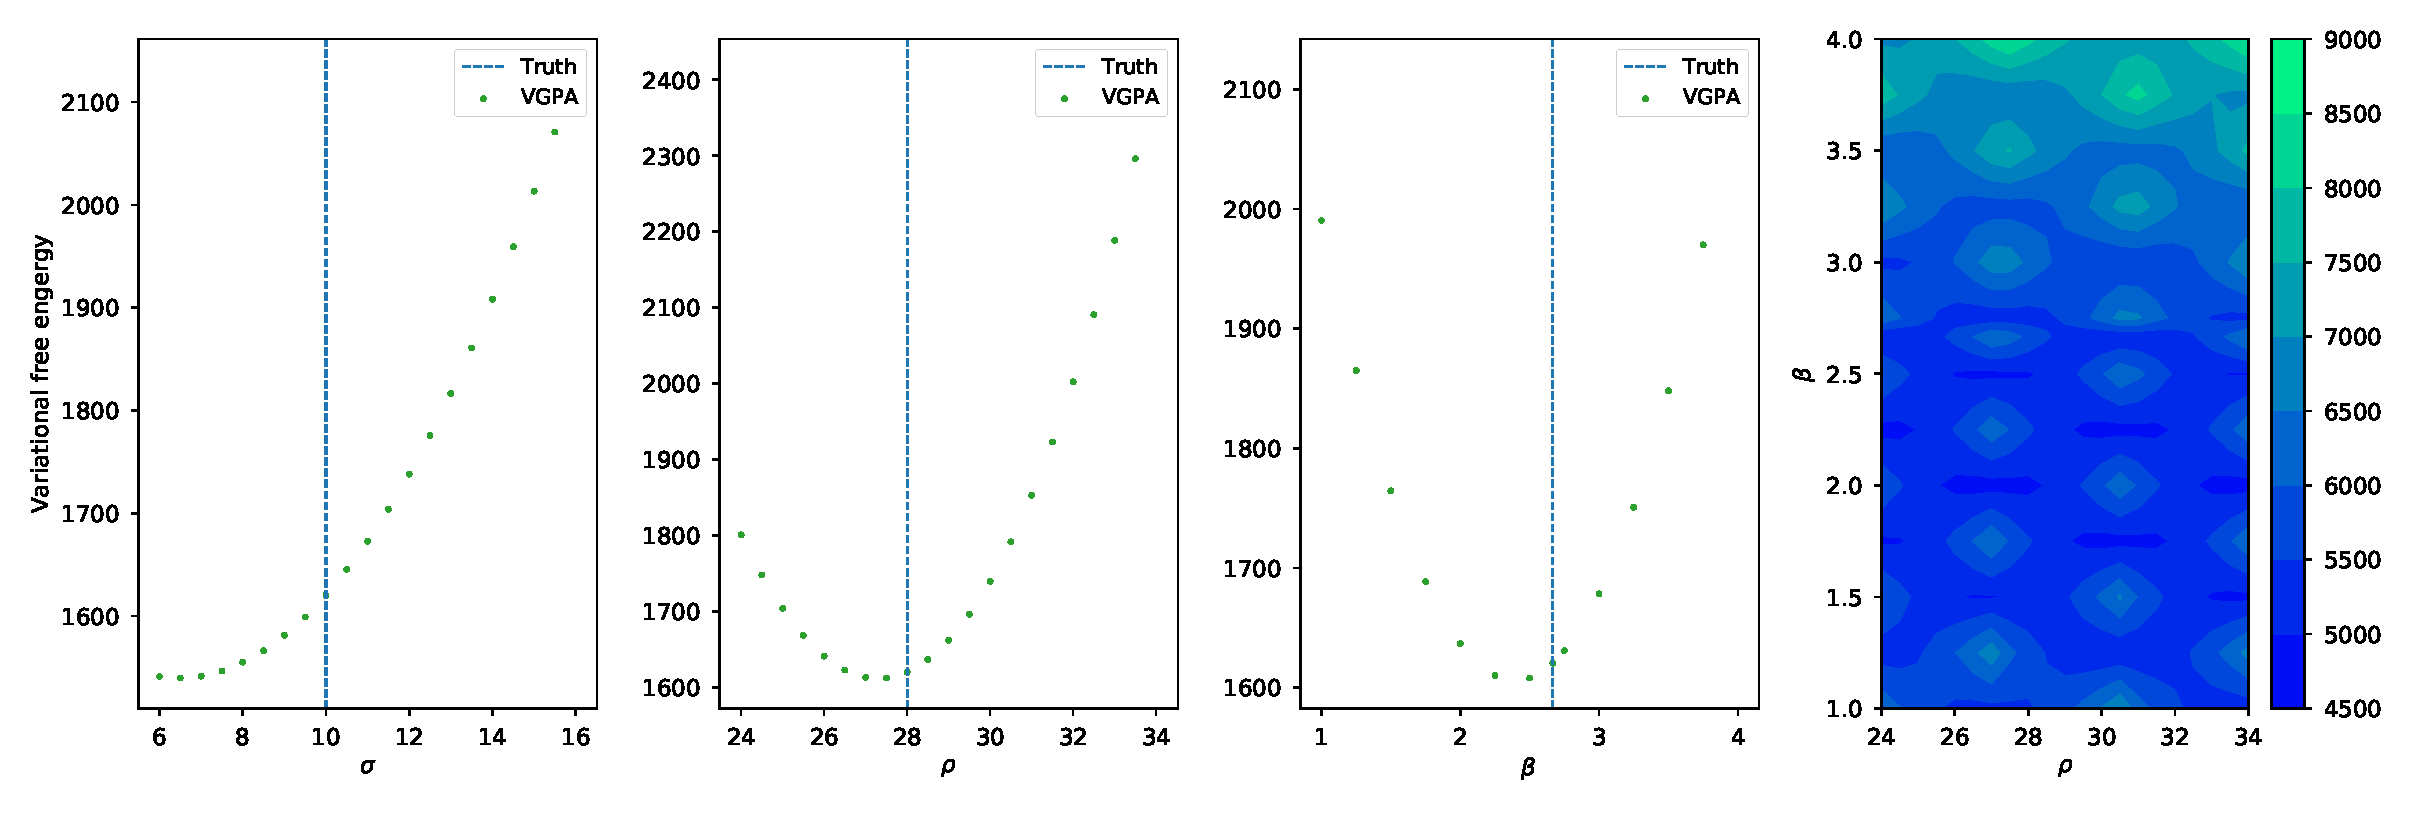
\includegraphics[width=\linewidth]{graphics/lorenz-63-parameters-grid-search}
    \caption{Grid search result using the \algovgpa\ algorithm for the stochastic Lorenz 63 model. The green dots indicate where the grid search is carried out, while the dash blue line indicates the true parameter value. The color map shows the existence of local minima when varying the parameters $\beta$ and $\rho$ together.}
    \label{fig-lorenz-63-parameters-grid-search}    
\end{figure}

\begin{figure}
    \centering
    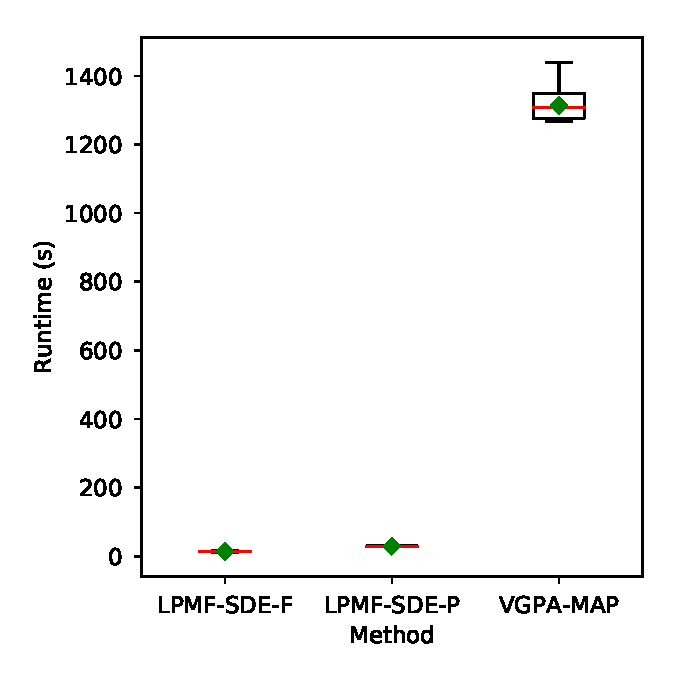
\includegraphics[width=0.48\linewidth]{graphics/lorenz-63-runtime-boxplot}
    \caption{Box plot for the runtimes over 10 repetitions using independent sample paths from the stochastic Lorenz 63 model. The median is indicated by the red line, while the mean is shown as the green diamond. The box shows the lower and upper quartiles, while the whiskers are the 5th and 95th percentiles.}
    \label{fig-lorenz-63-runtime-boxplot}    
\end{figure}

For parameter estimation, the results are presented in \reffigure{\ref{fig-lorenz-63-parameters-group}}.
Overall, the estimation based on both methods seem to be on par with each other with relatively low variance when all the states are observed.
Given that the \algovgpamap\ algorithm achieves better accuracy when estimating the states, it would be expected that the parameter estimation to also be better.
The non-optimal performance is probably due to the simple gradient update strategy as mentioned before.

If we look at \reffigure{\ref{fig-lorenz-63-parameters}} in detail, the large variance around the estimation for parameter $\sigma$ when state $y$ is unobserved is noticeable.
To explain this, first note that $\sigma$ appears only inside the first equation of \refequationp{\ref{eq-lorenz-63-odes}} together with state $x$ and $y$.
Since $y$ is not observable, the only source of information to estimate $\sigma$ is  $x$.
This is in contrast to the other two parameters $\rho$ and $\beta$, where both states $x$ and $z$ are used to estimate them.
Lastly, the means of the predicted parameters over the 10 independent runs are generally concentrated except for parameter $\rho$ inferred by the \algovgpamap\ algorithm, as shown in \reffigure{\ref{fig-lorenz-63-parameters-sigma-boxplot}} to \reffigure{\ref{fig-lorenz-63-parameters-rho-boxplot}}.

To further illustrate the difficulty of parameter estimation, grid search on the parameters is conducted using the original \algovgpa\ method.
Specifically, the step size used for the grid search is 0.5. 
The ranges for the searches for $\sigma, \rho, \beta$ are $[6, 16]$, $[24, 34]$ and $[1, 4]$ respectively.
Using the first plot in \reffigure{\ref{fig-lorenz-63-parameters-grid-search}} as an example, the changes in the variational free energy is plotted as the parameter $\sigma$ changes while the other two parameters are kept at the true values.
It can be seen that the parameter value that leads to the minimum of the variational free energy deviates from the true parameter values.
Moreover, the last plot in \reffigure{\ref{fig-lorenz-63-parameters-grid-search}} shows the existence of many local minima as we vary two parameters together, which makes parameter estimation based on grid search difficult.

\subsubsection*{Runtime performance}

\reffigure{\ref{fig-lorenz-63-runtime-boxplot}} shows the distribution of the average time to solve one RODE sample path and the runtime of the \algovgpamap\ algorithm to infer one SDE sample path after 10 independent repetitions. 
For each RODE sample, \algolpmfsde\ takes a fraction of the time required by \algovgpamap\ for one SDE sample path.
Even if the RODEs are not solved in parallel, the total runtime required by \algolpmfsde\ is still comparable to that of \algovgpamap. 
This further demonstrates the runtime efficiency of the \algolpmfsde\ scheme.

